\subsection{Paraview interactive based visualization}
When dealing with large scale simulation data, it might be inefficient to use Paraview client based visualization. One approach to visualize large scale data interactively is to run paraview in \texttt{client-server} mode. 
In \texttt{client-server} mode we can launch ParaView server (\texttt{pvserver}) using \texttt{MPI} and connect to that server through ParaView client. Above approach might be little hard to setup, and you need to run \texttt{pvserver} in 
exisiting supercomputer compute nodes, which cost critical amount of core hours. We have performed interactive \texttt{client-server} visualization in Utah's CHPC cluster. 

\subsection{Paraview batch mode based visualization}
ParaView batch mode visualization is same as the above \texttt{client-server} visualization except we use ParaView python wrapper to write code to generate specific views, and save images for each time step. This approach does not require 
ParaView GUI (i.e. all the pipeline setup is performed through ParaView python wrapper), and we can use configure flags to run ParaView in \texttt{offscreen-rendering} mode, hence easy to setup. In order to run ParaView in batch mode, 
we can use \texttt{pvbatch} which automatically does the client server setup based on the number of \texttt{MPI} tasks specified. For example if you want to run ParaView in $280$ cores in $10$ nodes in CHPC you can request $10$
compute nodes and launch the batch with offscreen rendering as follows. 

\begin{lstlisting}[basicstyle=\small]
mpirun -np 280 -N 28 pvbatch --use-offscreen-rendering <paraview python script>
\end{lstlisting}

Following are the main parts for the praview python script. The reading the \texttt{.pvtu} can be performed as following. 

\begin{lstlisting}[basicstyle=\small]
filename=[file_prefix+'_'+str(step)+'.pvtu']
print "reading: %s" %(filename)
# create a new 'XML Partitioned Unstructured Grid Reader'
pvtu = XMLPartitionedUnstructuredGridReader(FileName=filename)
# only selecting the variables that needed for the visualization.
pvtu.CellArrayStatus = ['cell_level'] 
pvtu.PointArrayStatus = ['U_ALPHA', 'U_CHI', 'U_K']

UpdatePipeline()
print "reading ended"
\end{lstlisting}

Then we need to generate the slice based on the \texttt{maxDepth} parameter which determined the slice origin due to how the simulation is setup and color by the variable $\chi$. 

\begin{lstlisting}[basicstyle=\small]
maxDepth=12; #max depth of the underlying octree. 
bh_range_min=-200
bh_range_max=200    # bh computational domain

CHI_FLOOR=0.1 # value to set scale for color bar
varName='U_CHI' # variable name to visualize

s_x=(1<<(maxDepth-1))
s_y=(1<<(maxDepth-1))
s_z=(1<<(maxDepth-1))
scale_factor=2048.0

# create a new 'Slice'
pvtu_slice = Slice(Input=pvtu)
pvtu_slice.SliceType = 'Plane'
pvtu_slice.SliceOffsetValues = [0.0]
  
# set the slice origin
pvtu_slice.SliceType.Origin = [s_x, s_y, s_z]
  
# Properties modified on slice1.SliceType
pvtu_slice.SliceType.Normal = [0.0, 0.0, 1.0]
# set to don't triangualte the slice since we are using the the octree mesh. 
pvtu_slice.Triangulatetheslice = 0
  
print "slice created"
UpdatePipeline()
print "pipeline updated"
# show data in view
slice_display = Show(pvtu_slice, renderView1)
# trace defaults for the display properties.
slice_display.ColorArrayName = [None, '']

ColorBy(slice_display, ('POINTS', varName))
 
uCHILUT = GetColorTransferFunction(varName)
uCHIPWF = GetOpacityTransferFunction(varName)
 
uCHILUT.ColorSpace = 'Diverging'
uCHILUT.NumberOfTableValues = 1024
u_CHILUTColorBar = GetScalarBar(uCHILUT, renderView1)
u_CHILUTColorBar.Title = varName
u_CHILUTColorBar.ComponentTitle = ''
u_CHILUTColorBar.TitleJustification = 'Centered'
 
uCHILUT.RescaleTransferFunction(CHI_FLOOR, 1.0)
uCHIPWF.RescaleTransferFunction(CHI_FLOOR, 1.0)
slice_display.SetScalarBarVisibility(renderView1, False)
 
UpdatePipeline()
renderView1.Update()
\end{lstlisting}

Then we perform the the same operations for the times series data which is performed by,
\begin{lstlisting}[basicstyle=\small]
step_begin=int(args['begin'])
step_end=int(args['end'])
step_freq=int(args['freq'])
file_prefix=args['pvtu_prefix']
img_prefix=args['img_prefix']

n_procs = servermanager.vtkProcessModule.GetProcessModule().GetNumberOfLocalPartitions()
print "number of ranks: ", n_procs
imgCount=step_begin/step_freq;

for step in range(step_begin,step_end,step_freq):
saveImg(file_prefix,img_prefix,step,imgCount)
imgCount=imgCount+1;
\end{lstlisting}

Note that in paraview \texttt{XMLPartitionedUnstructuredGridReader} by construction is desined to use parallel processing for generate filters and parallel rendering. 


For the ParaView batch mode based visualization we have generated $4$ images for each timestep for black hole merger simulation of mass ratios $1,10$ and $100$. 
\begin{itemize}
    \item Compute a slice through the black hole plane and color them by the BSSN variable $\chi$
    \item Visualize the same slice with the underling AMR mesh structure (i.e. refinement level) $cell\_level$    
    \item Compute warp by scalr based on $\chi$ with scale factor of $100$ in $(0,0,1)$ direction
    \item Visualize the warped slice with the underling grid structure. 
\end{itemize}

Above simulations are mainly interesting since BSSN variable $\chi$ can be use to identify the each singularity in spacetime, and cell structure is important to check the Adaptive Mesh Refinement (AMR) is functioning properly. Few of the generated
images are shown in Figures \ref{fig:pv:r1},\ref{fig:pv:r10} and \ref{fig:pv:r100} 

\begin{figure}[H]
    \centering
    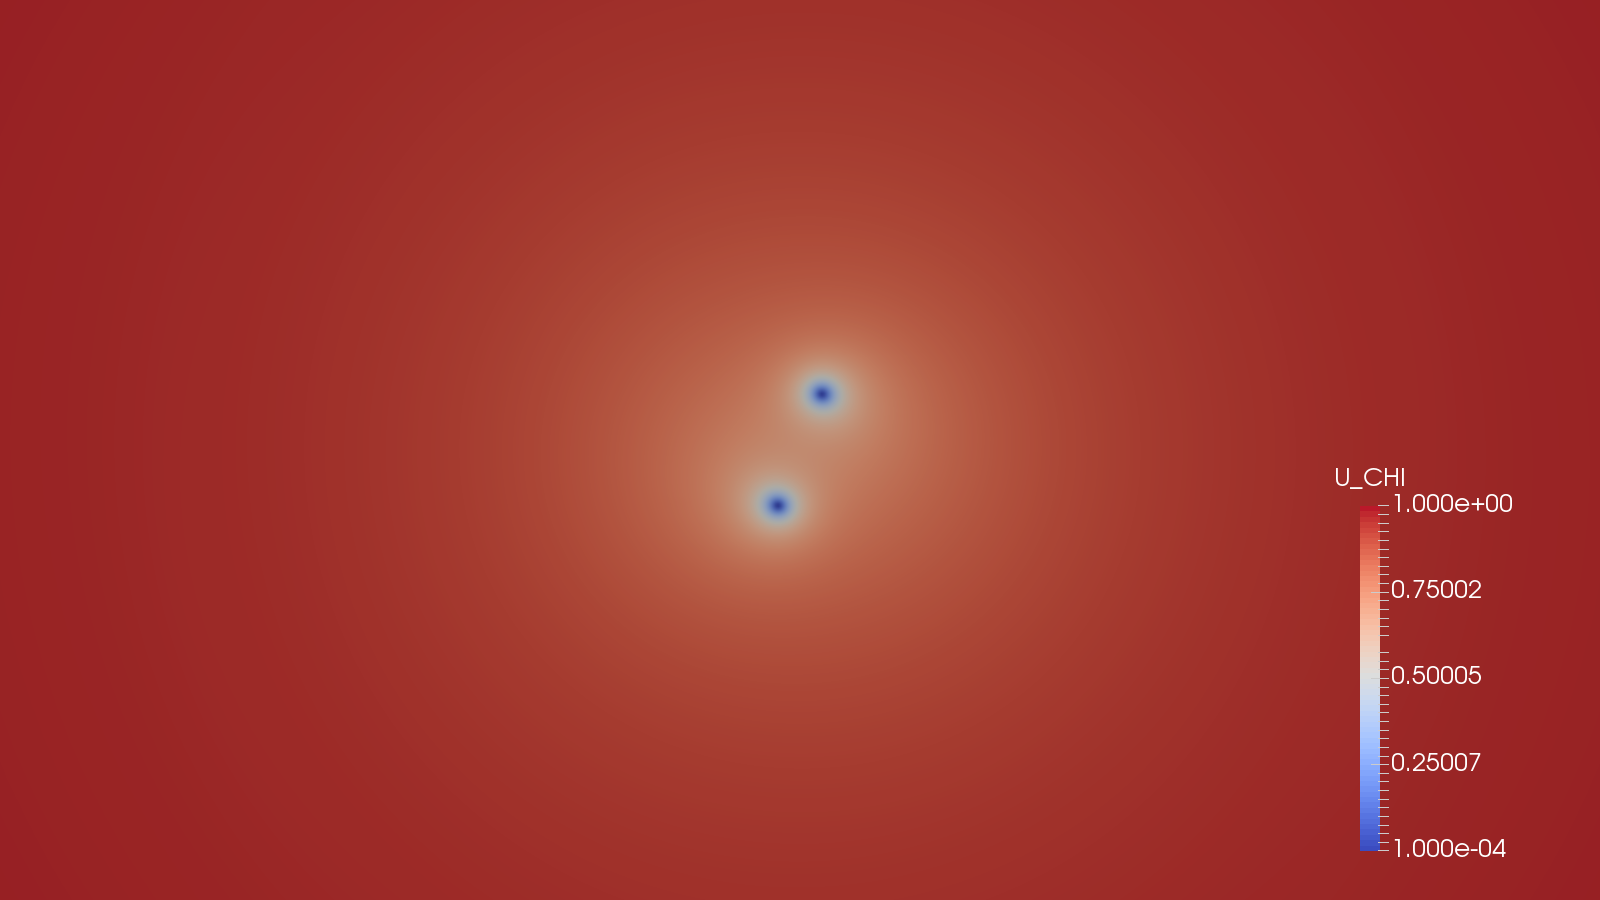
\includegraphics[width=0.22\textwidth]{figs/paraview/r1/img_slice_000200.png}
    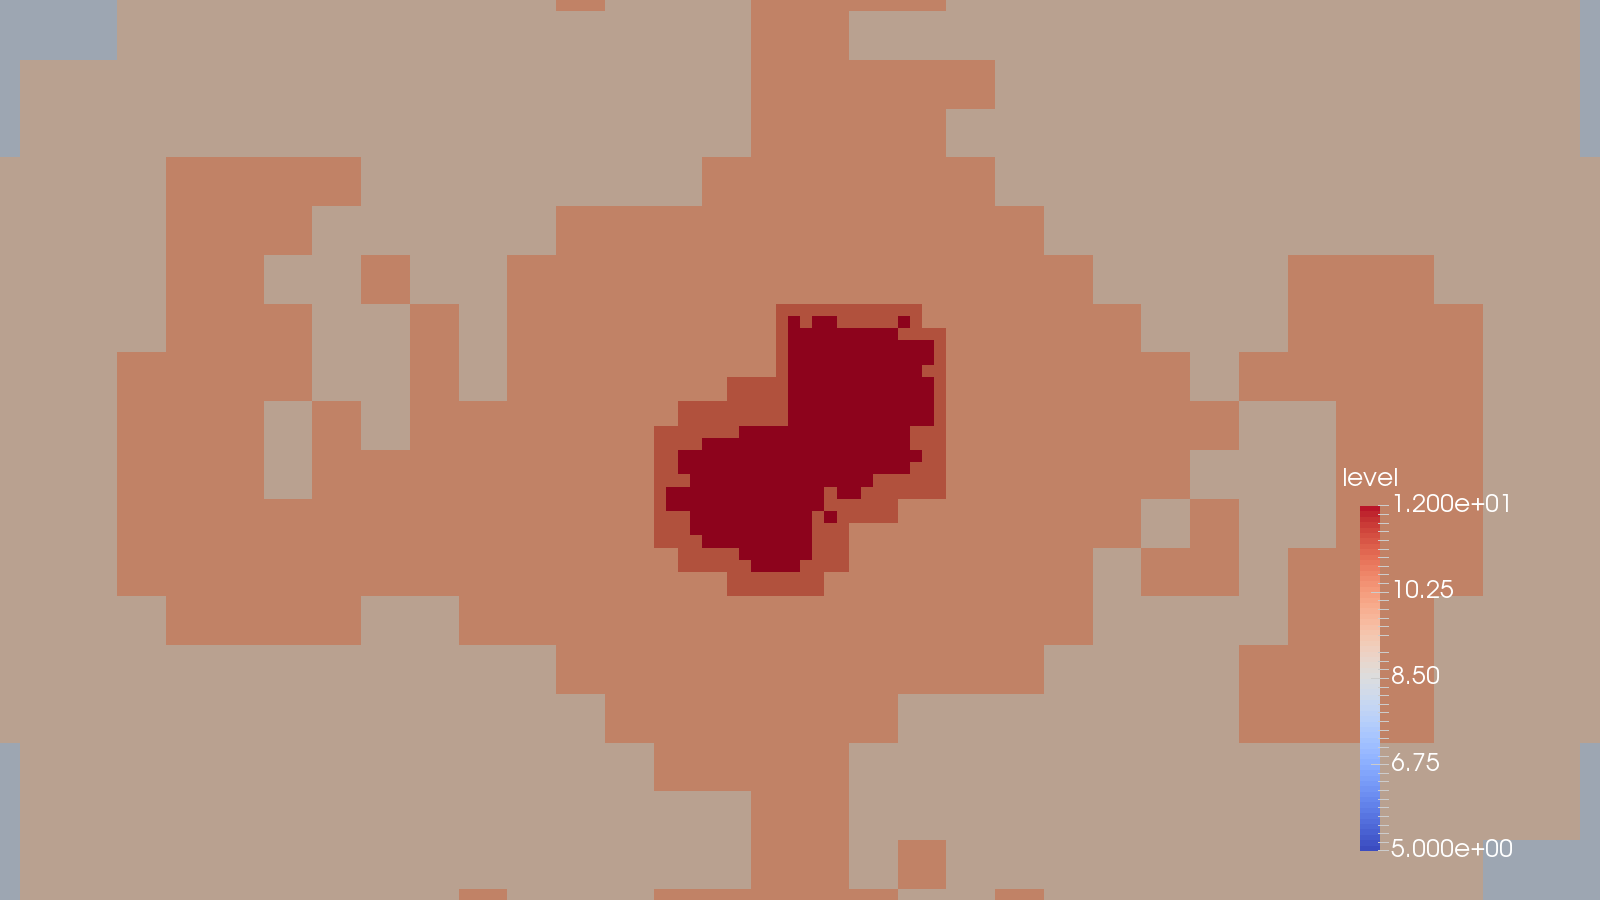
\includegraphics[width=0.22\textwidth]{figs/paraview/r1/img_slice_level_000200.png}
    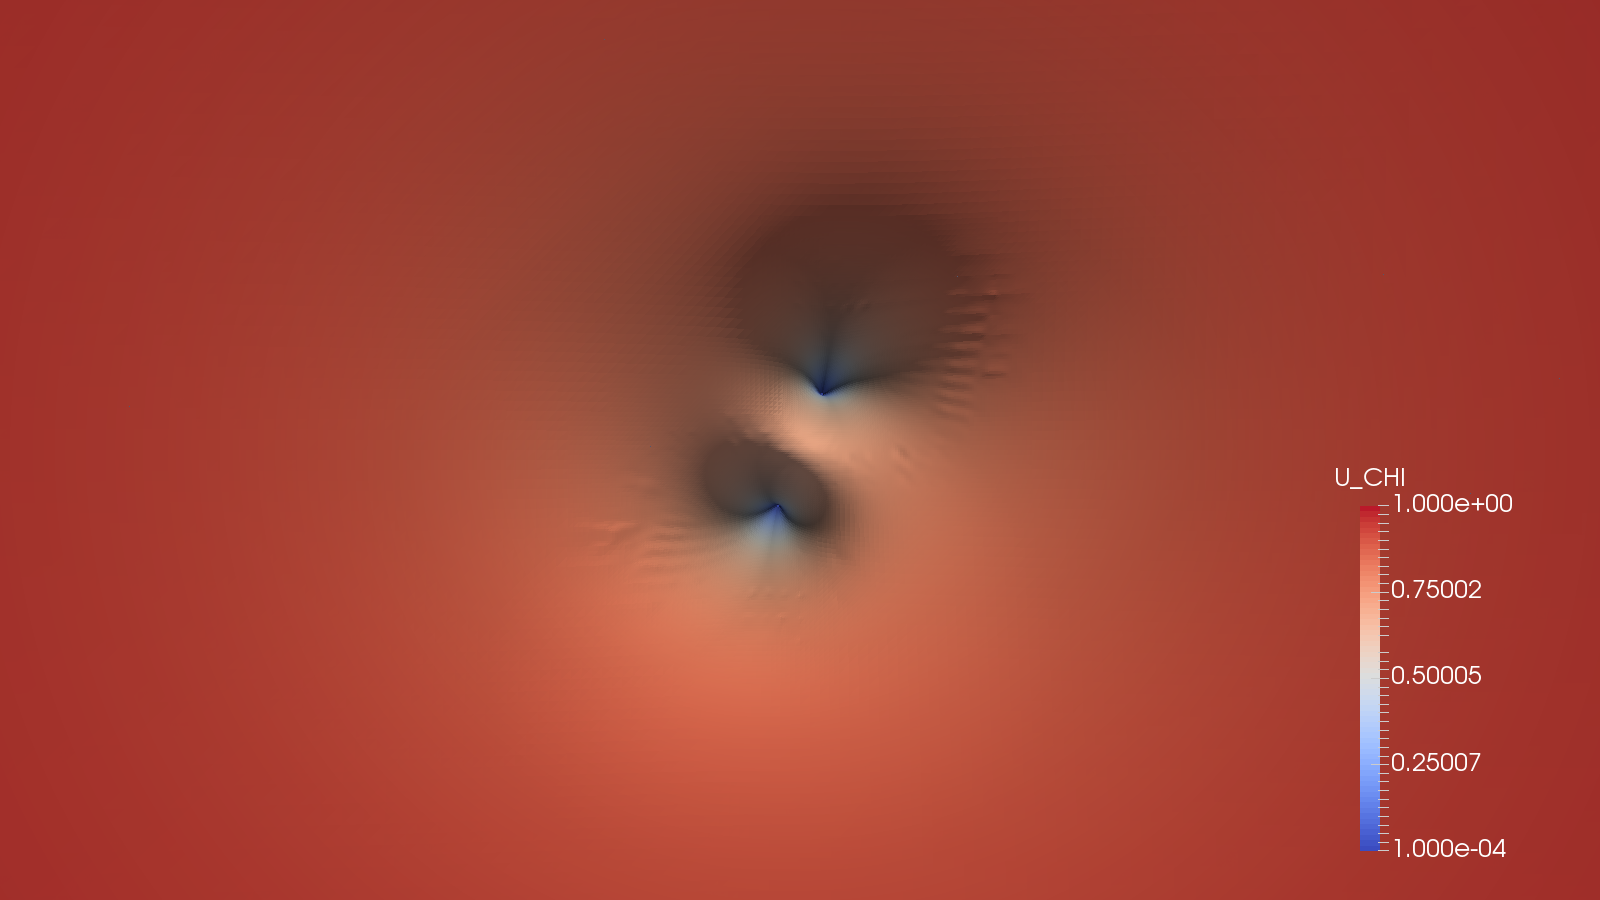
\includegraphics[width=0.22\textwidth]{figs/paraview/r1/img_slice_wbs_000200.png}
    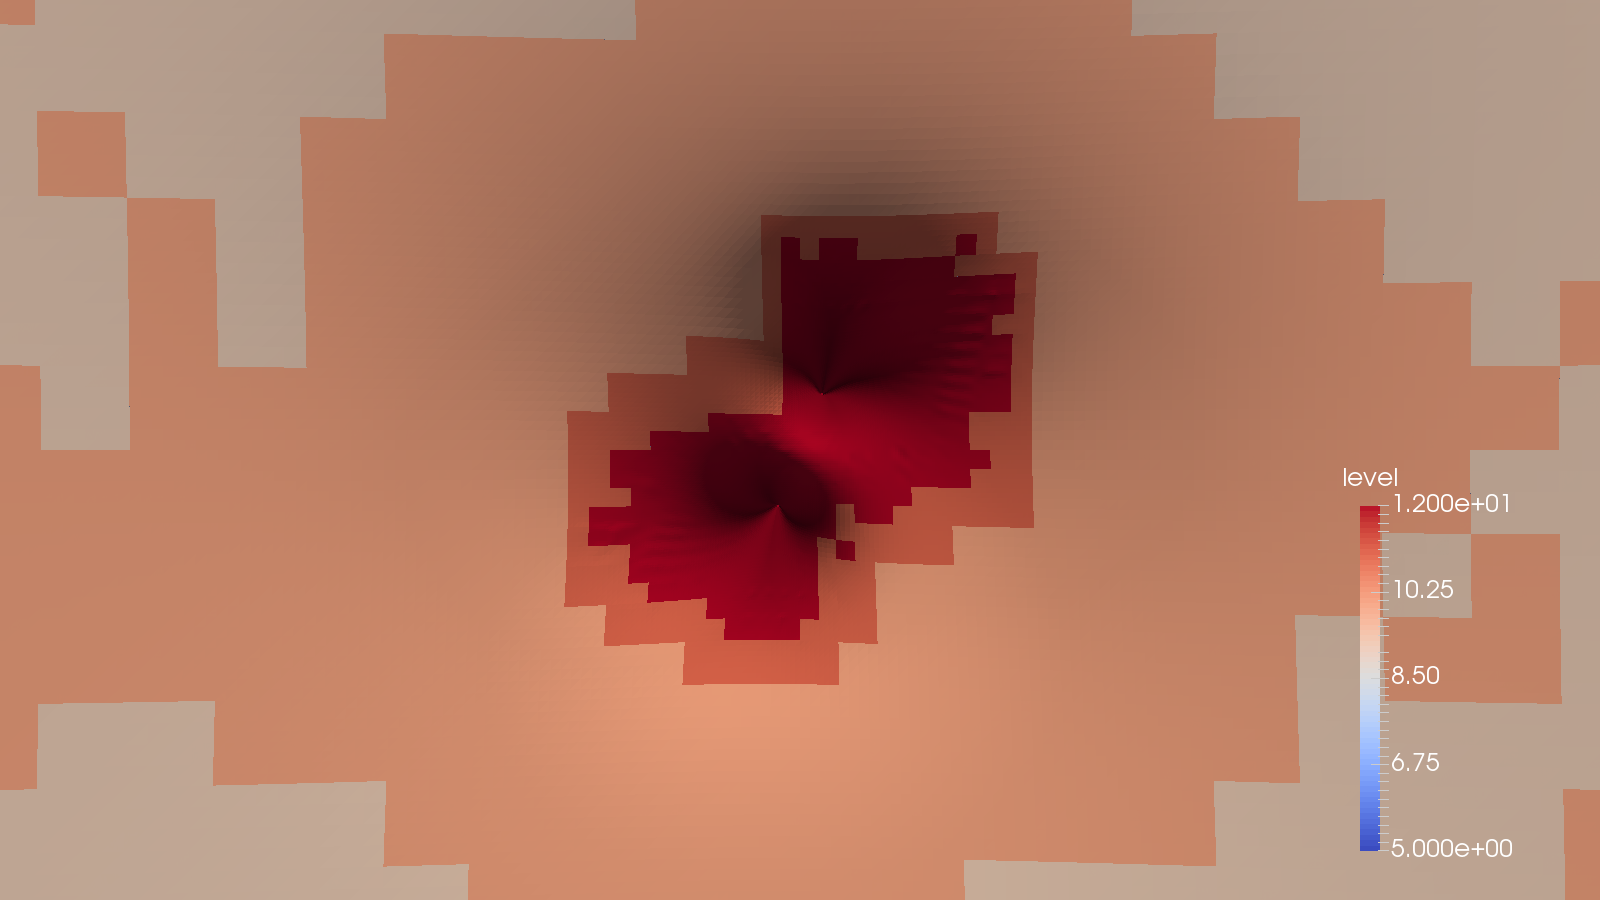
\includegraphics[width=0.22\textwidth]{figs/paraview/r1/img_slice_level_wbs_000200.png}
    \caption{Equal mass ratio black hole merger simulation with maximum refinement level of $12$ with wavelet tolerance of $10^{-4}$ perfomred in CHPC \label{fig:pv:r1}}
\end{figure}


\begin{figure}[H]
    \centering
    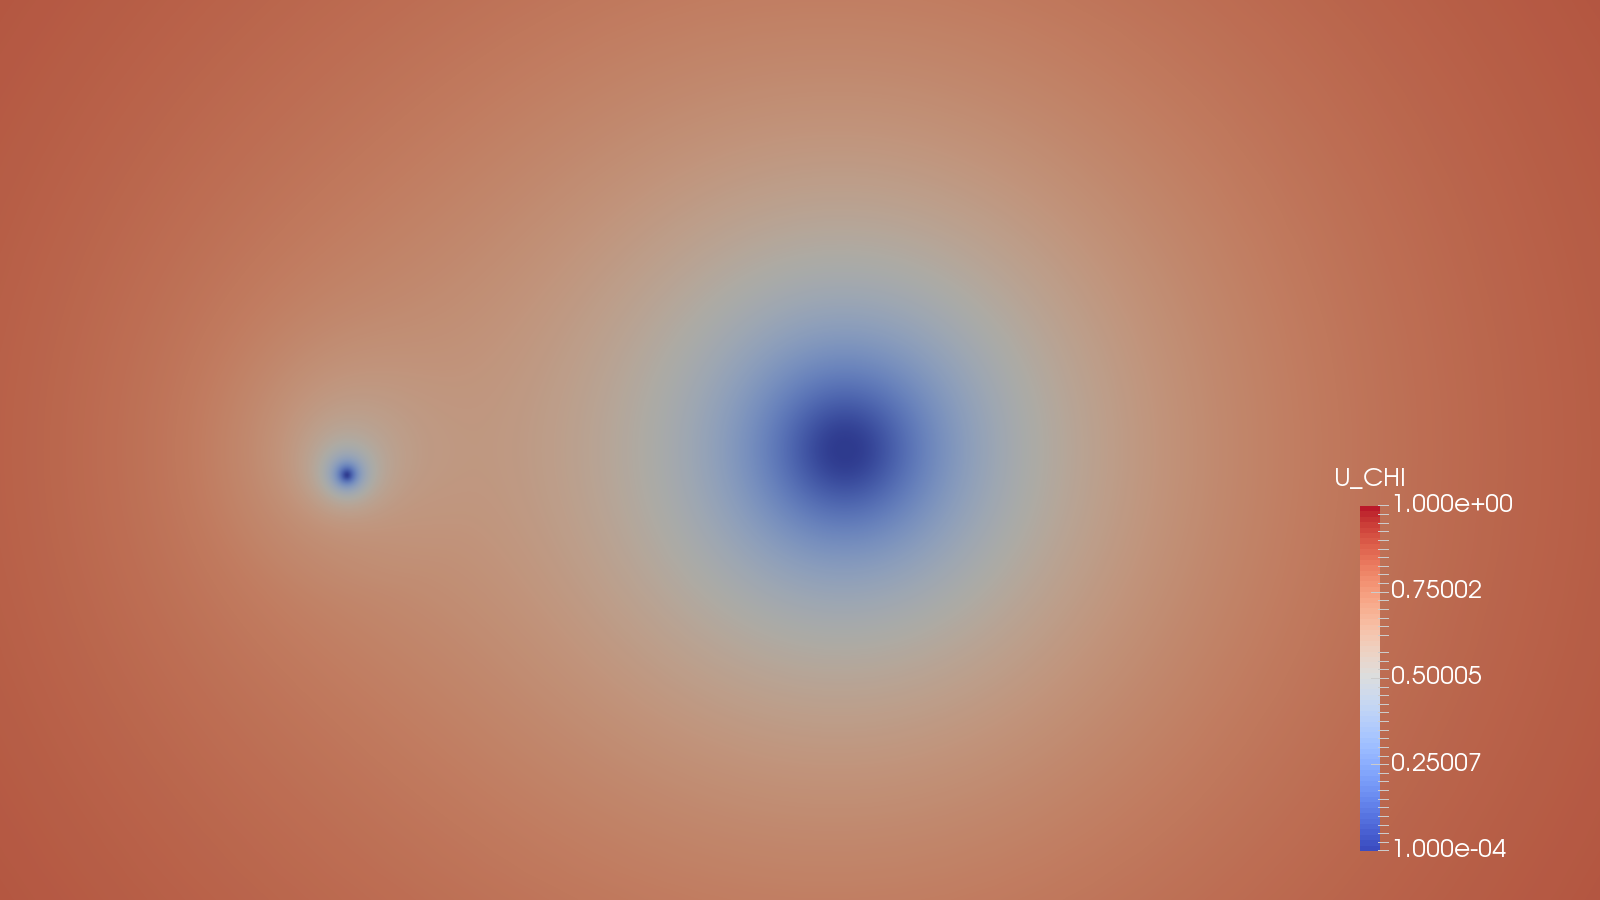
\includegraphics[width=0.22\textwidth]{figs/paraview/r10/img_slice_000050.png}
    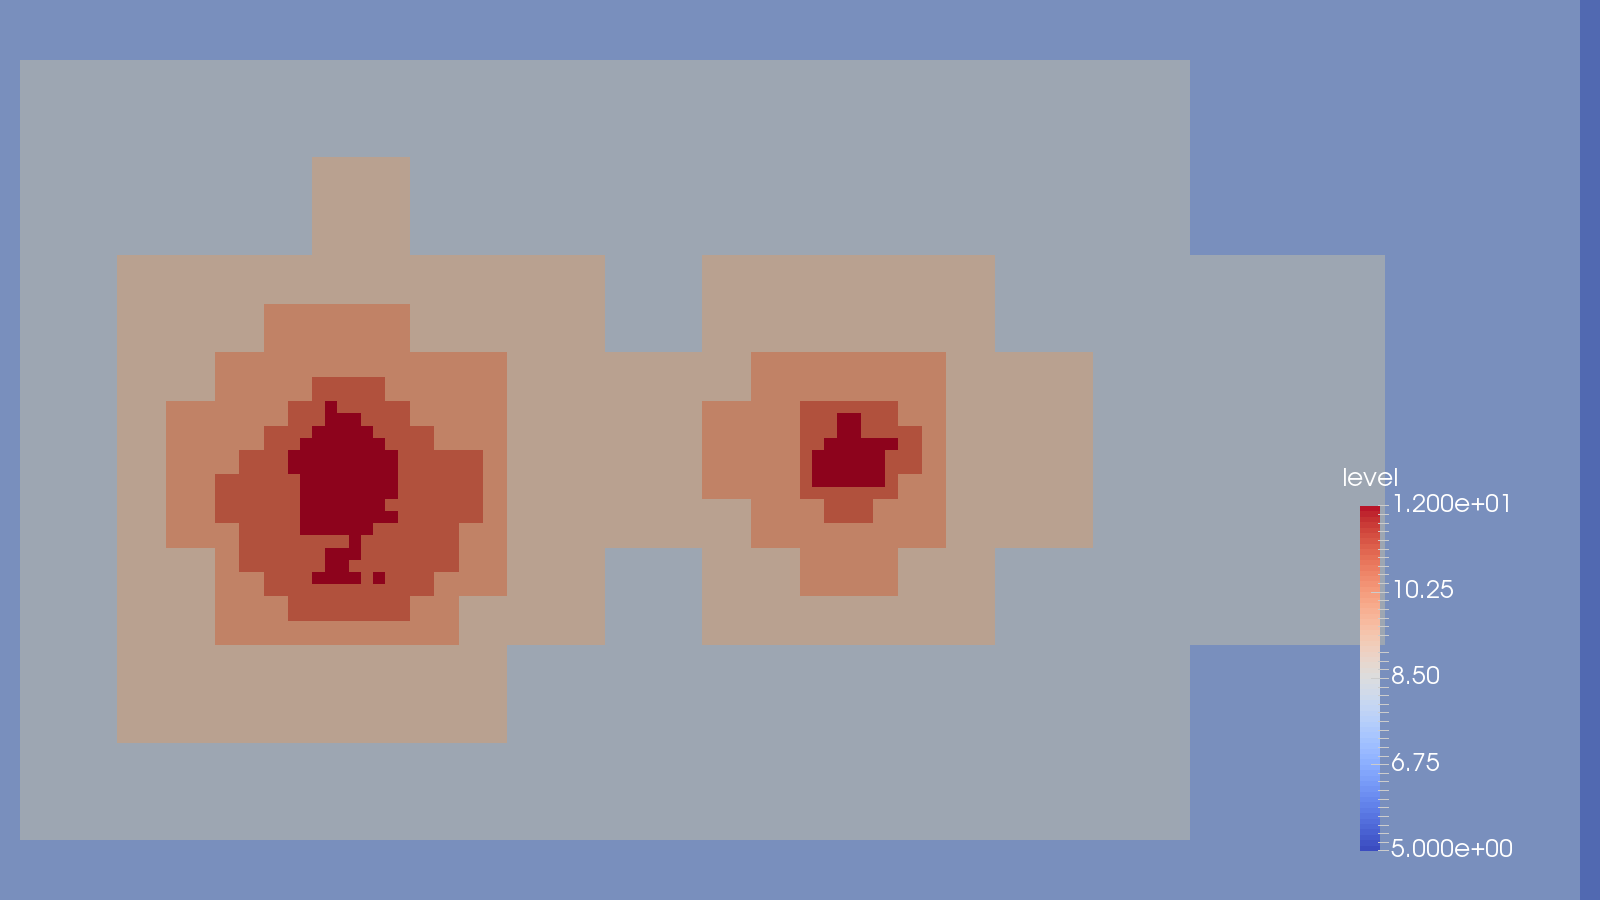
\includegraphics[width=0.22\textwidth]{figs/paraview/r10/img_slice_level_000050.png}
    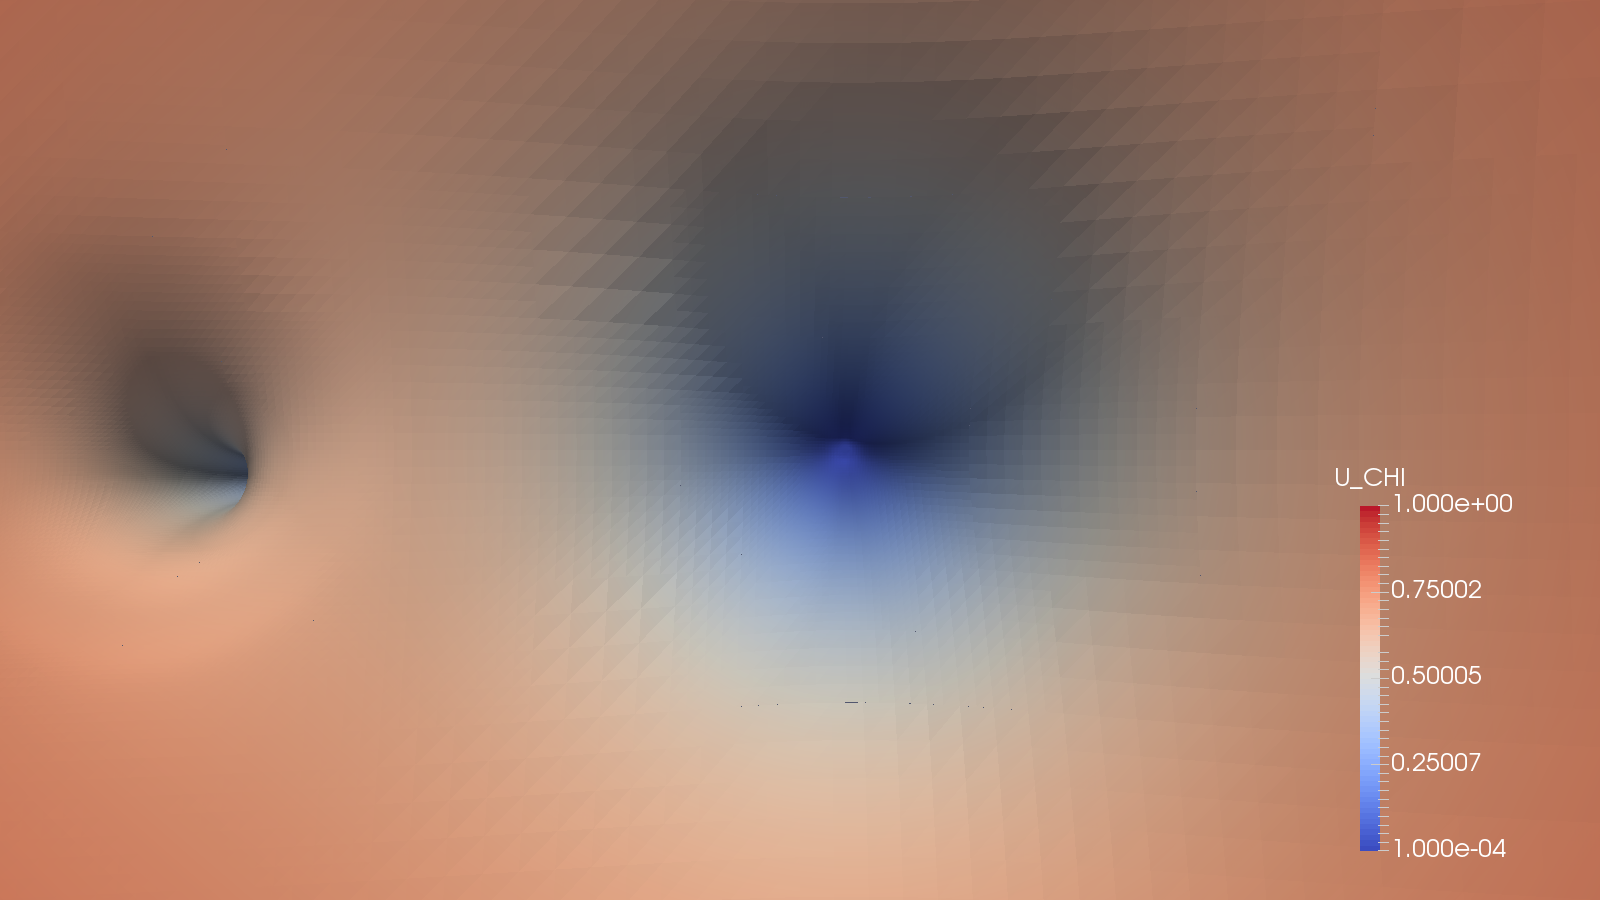
\includegraphics[width=0.22\textwidth]{figs/paraview/r10/img_slice_wbs_000050.png}
    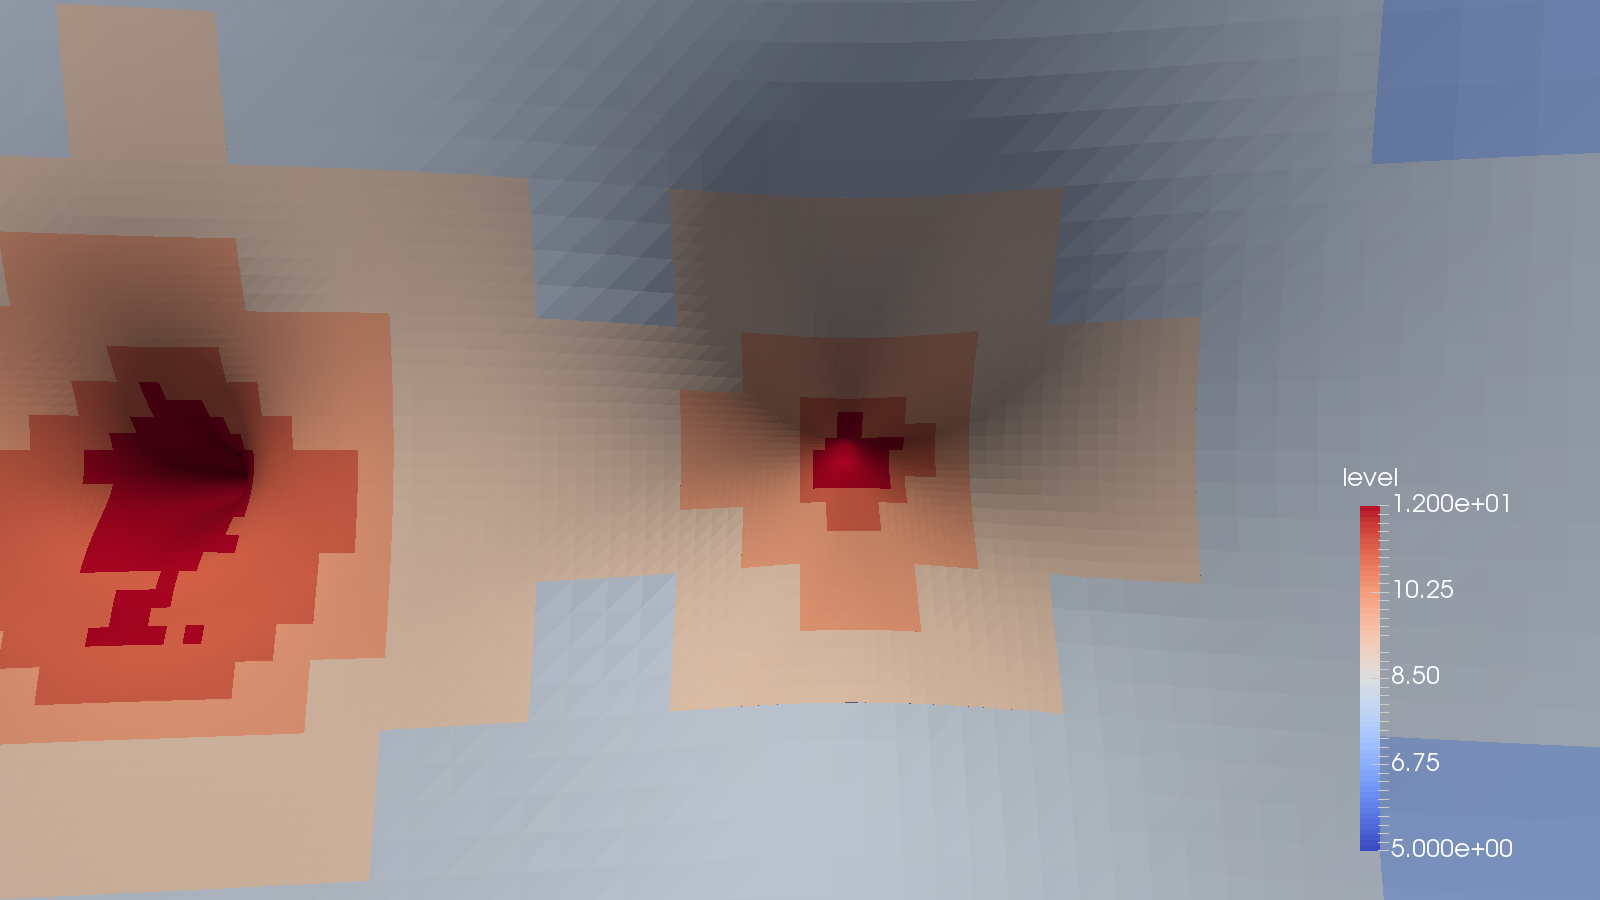
\includegraphics[width=0.22\textwidth]{figs/paraview/r10/img_slice_level_wbs_000050.png}
    \caption{Mass ratio of 10 black hole merger simulation with maximum refinement level of $12$ with wavelet tolerance of $10^{-4}$ perfomred in CHPC \label{fig:pv:r10}}
\end{figure}


\begin{figure}[H]
    \centering
    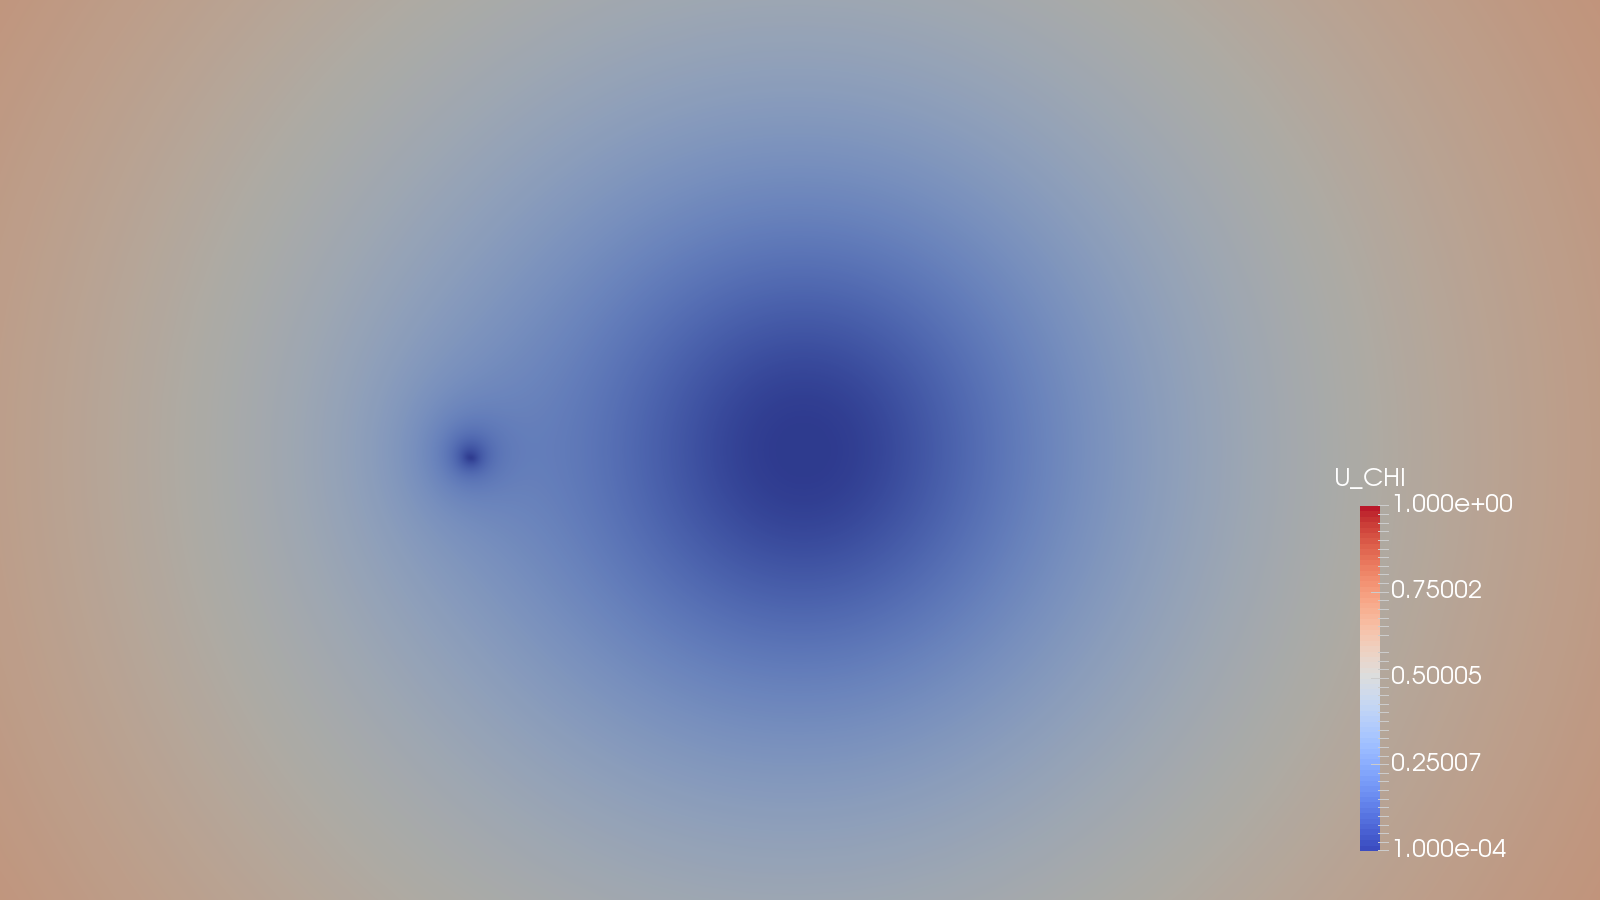
\includegraphics[width=0.22\textwidth]{figs/paraview/r100/img_slice_000050.png}
    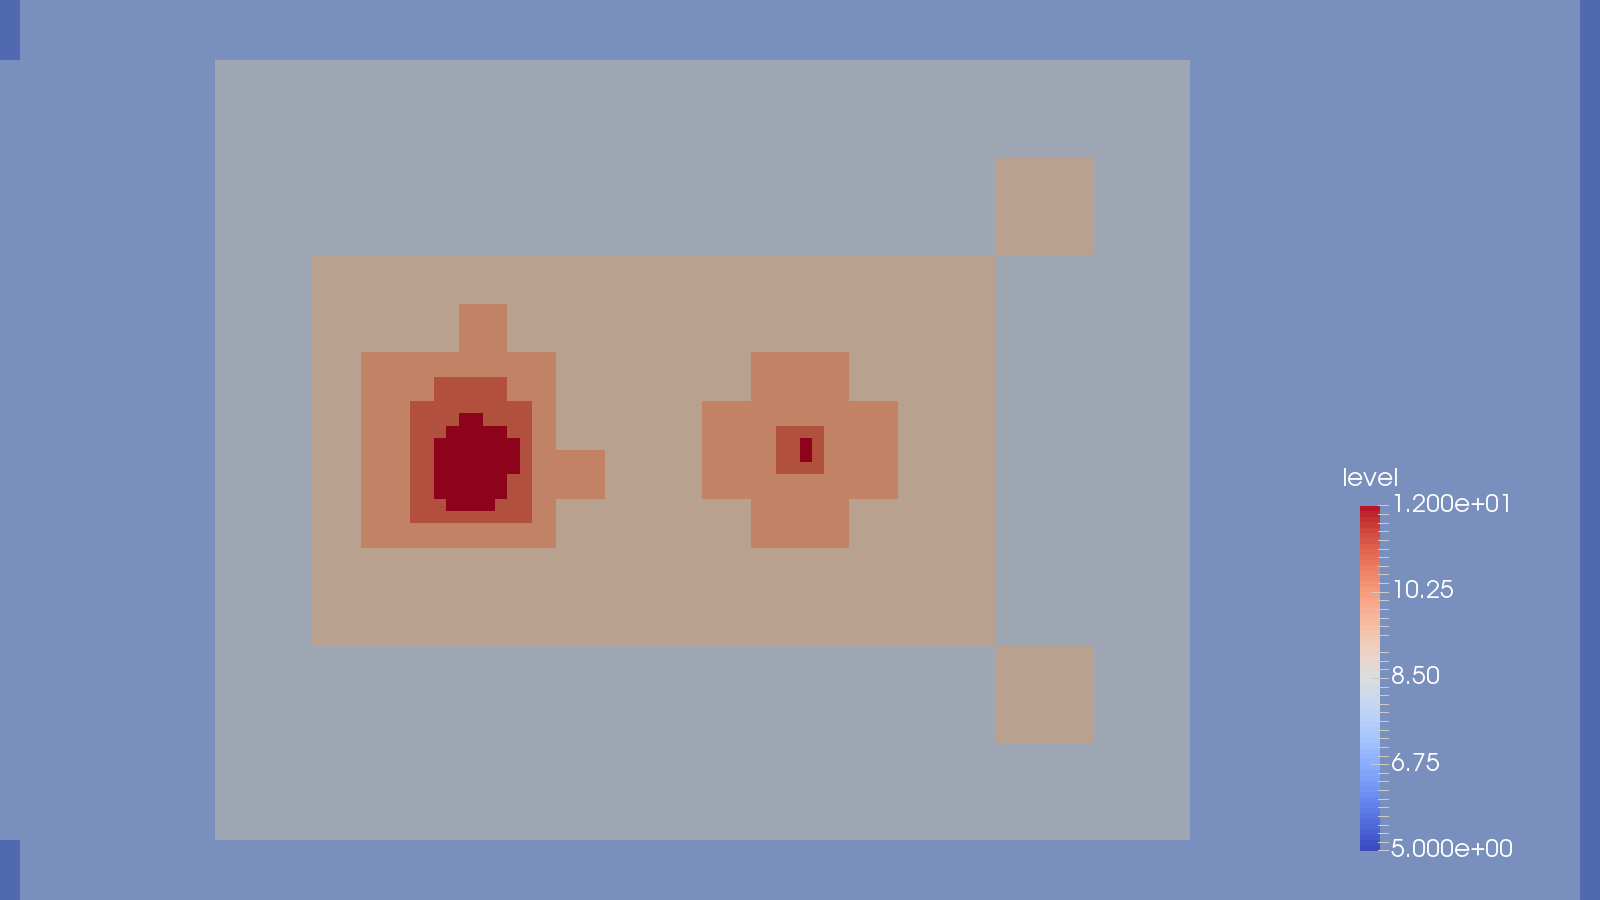
\includegraphics[width=0.22\textwidth]{figs/paraview/r100/img_slice_level_000050.png}
    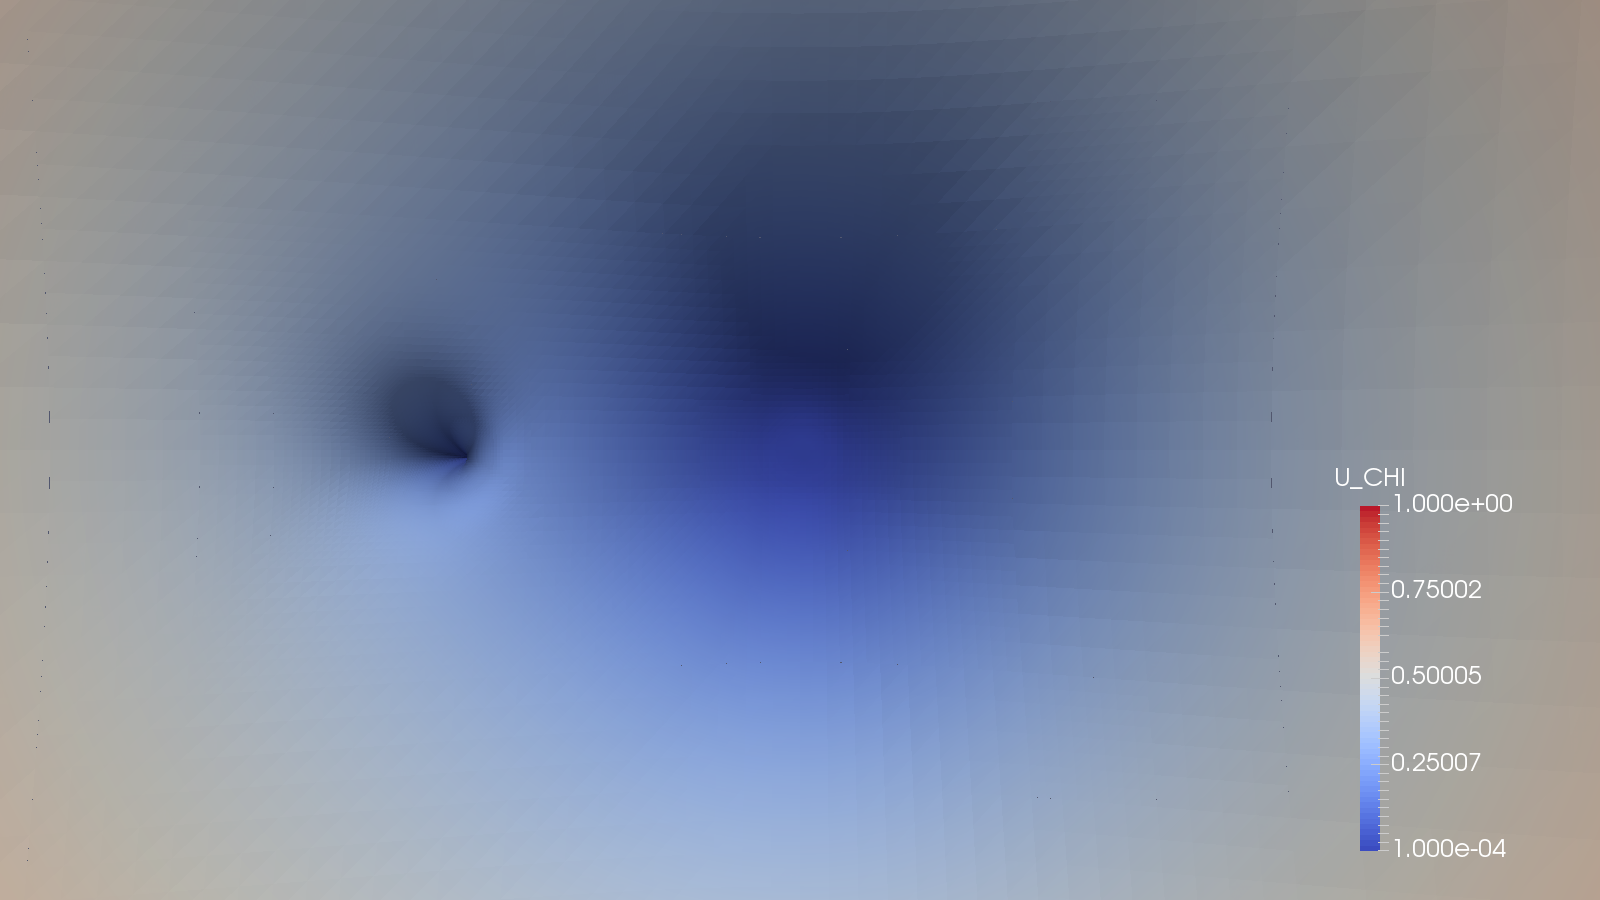
\includegraphics[width=0.22\textwidth]{figs/paraview/r100/img_slice_wbs_000050.png}
    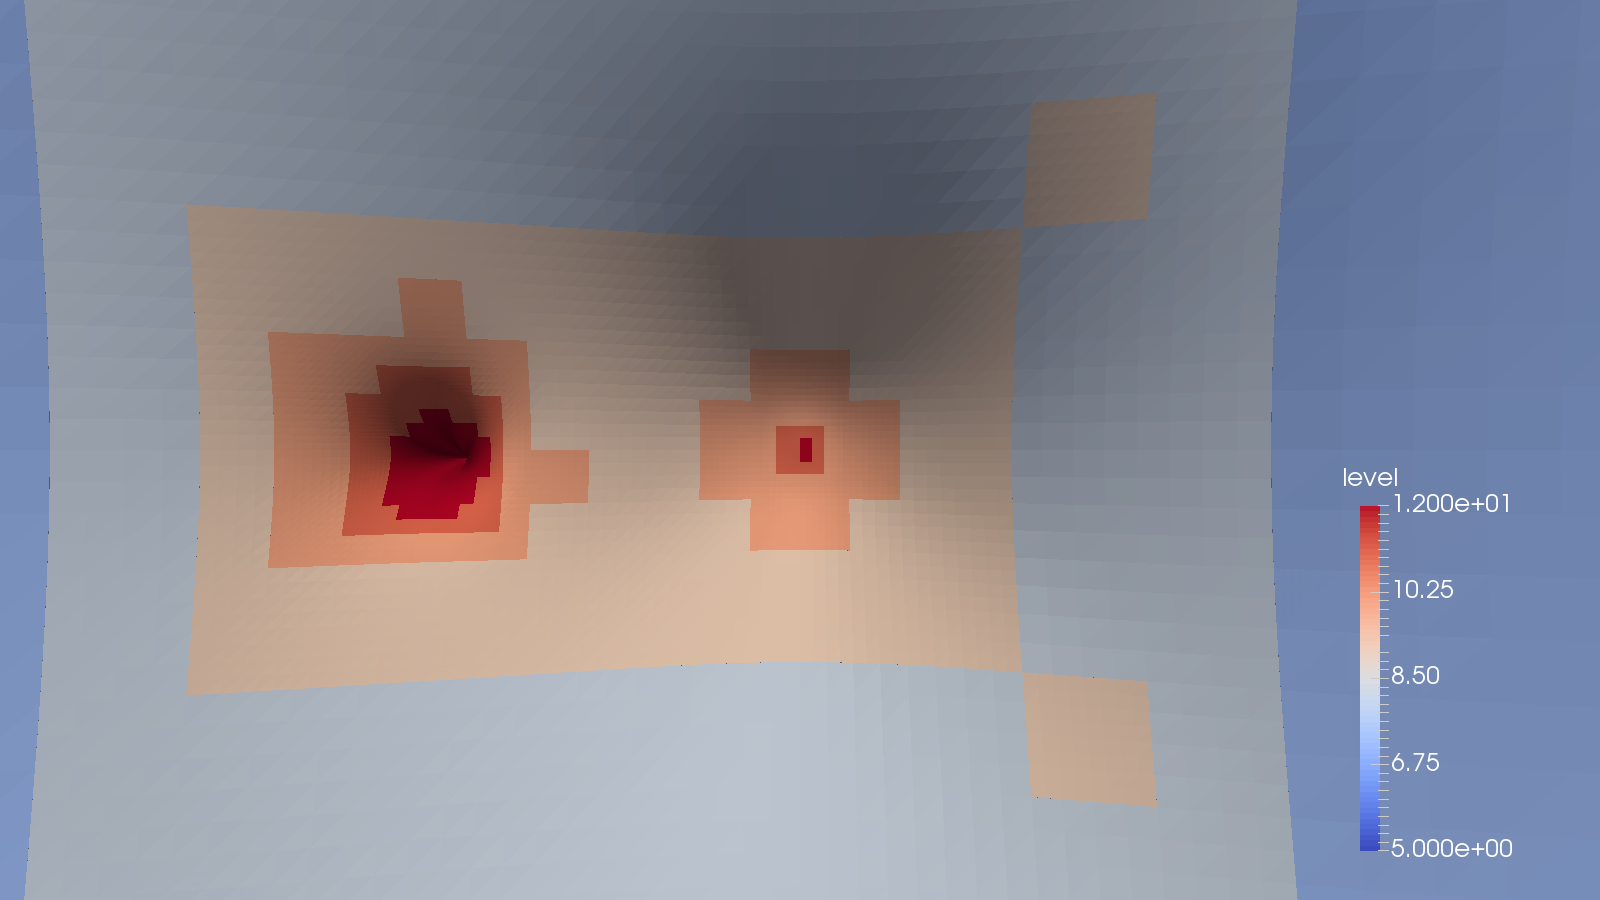
\includegraphics[width=0.22\textwidth]{figs/paraview/r100/img_slice_level_wbs_000050.png}
    \caption{Mass ratio of 100 black hole merger simulation with maximum refinement level of $12$ with wavelet tolerance of $10^{-4}$ perfomred in CHPC \label{fig:pv:r100}}
\end{figure}



\begin{figure}[H]
	\centering
	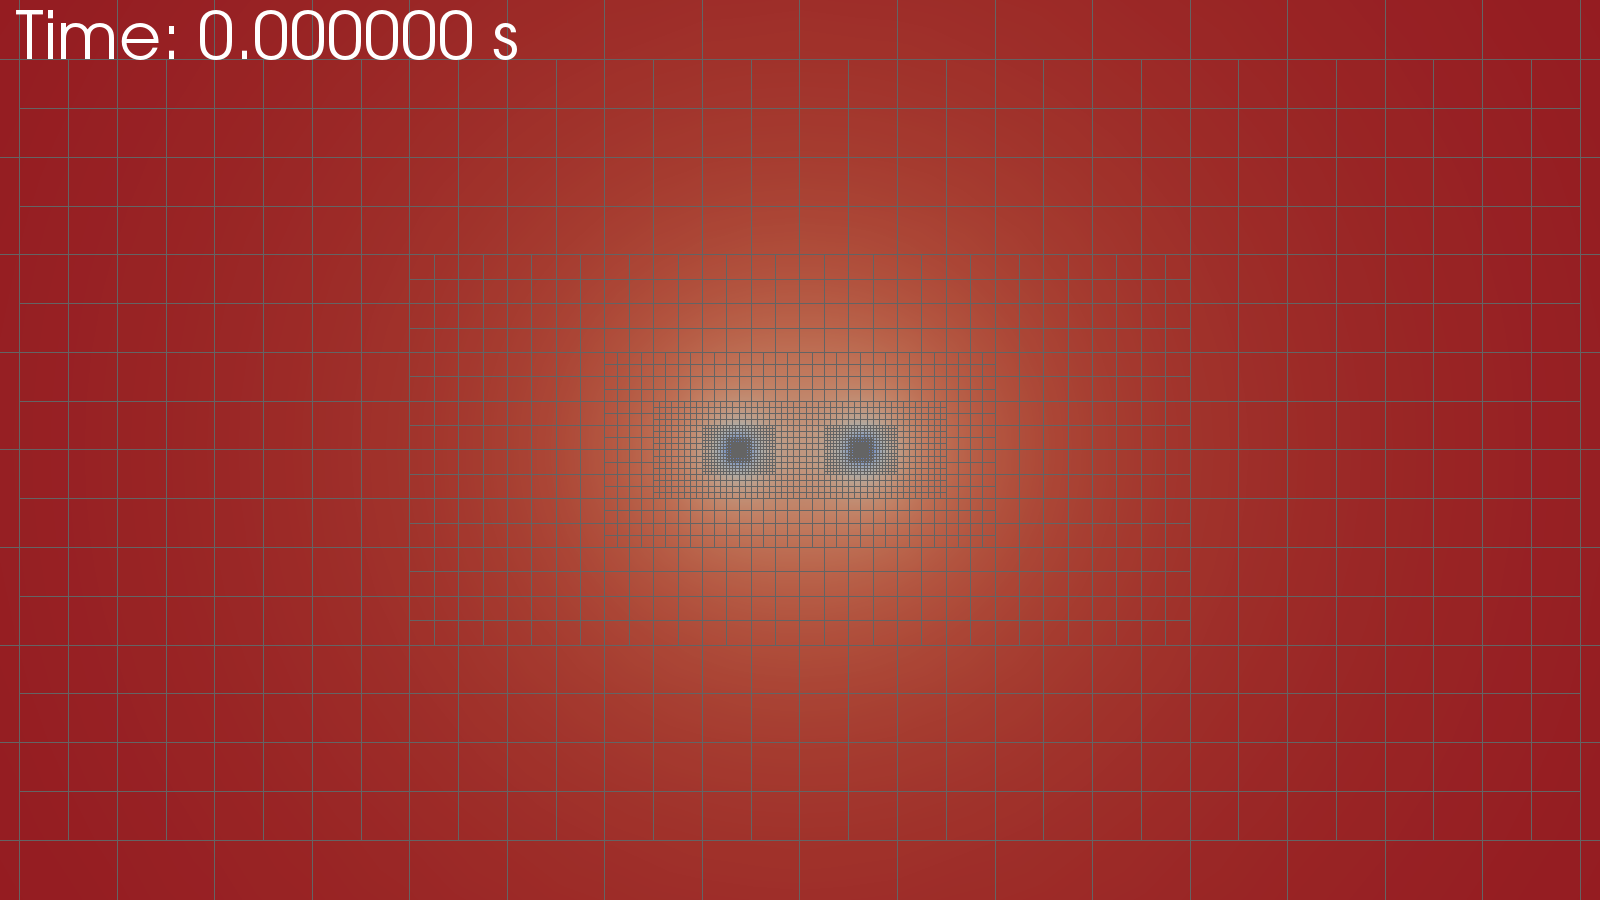
\includegraphics[width=0.22\textwidth]{figs/paraview/r1/new/img_slice_level_000000.png}
	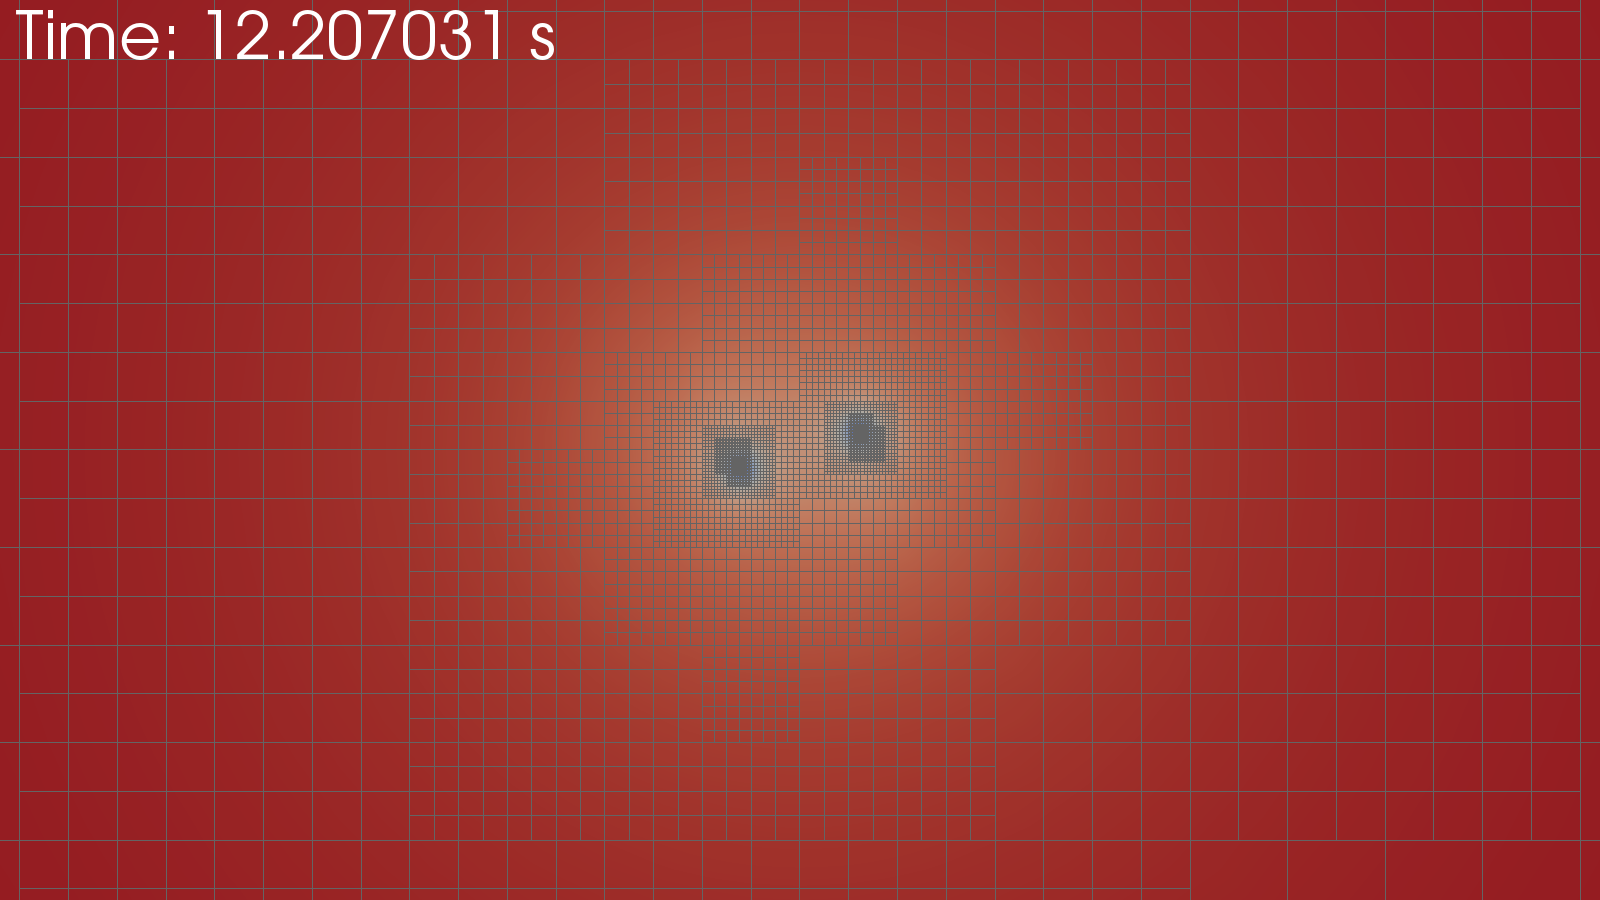
\includegraphics[width=0.22\textwidth]{figs/paraview/r1/new/img_slice_level_000100.png}
	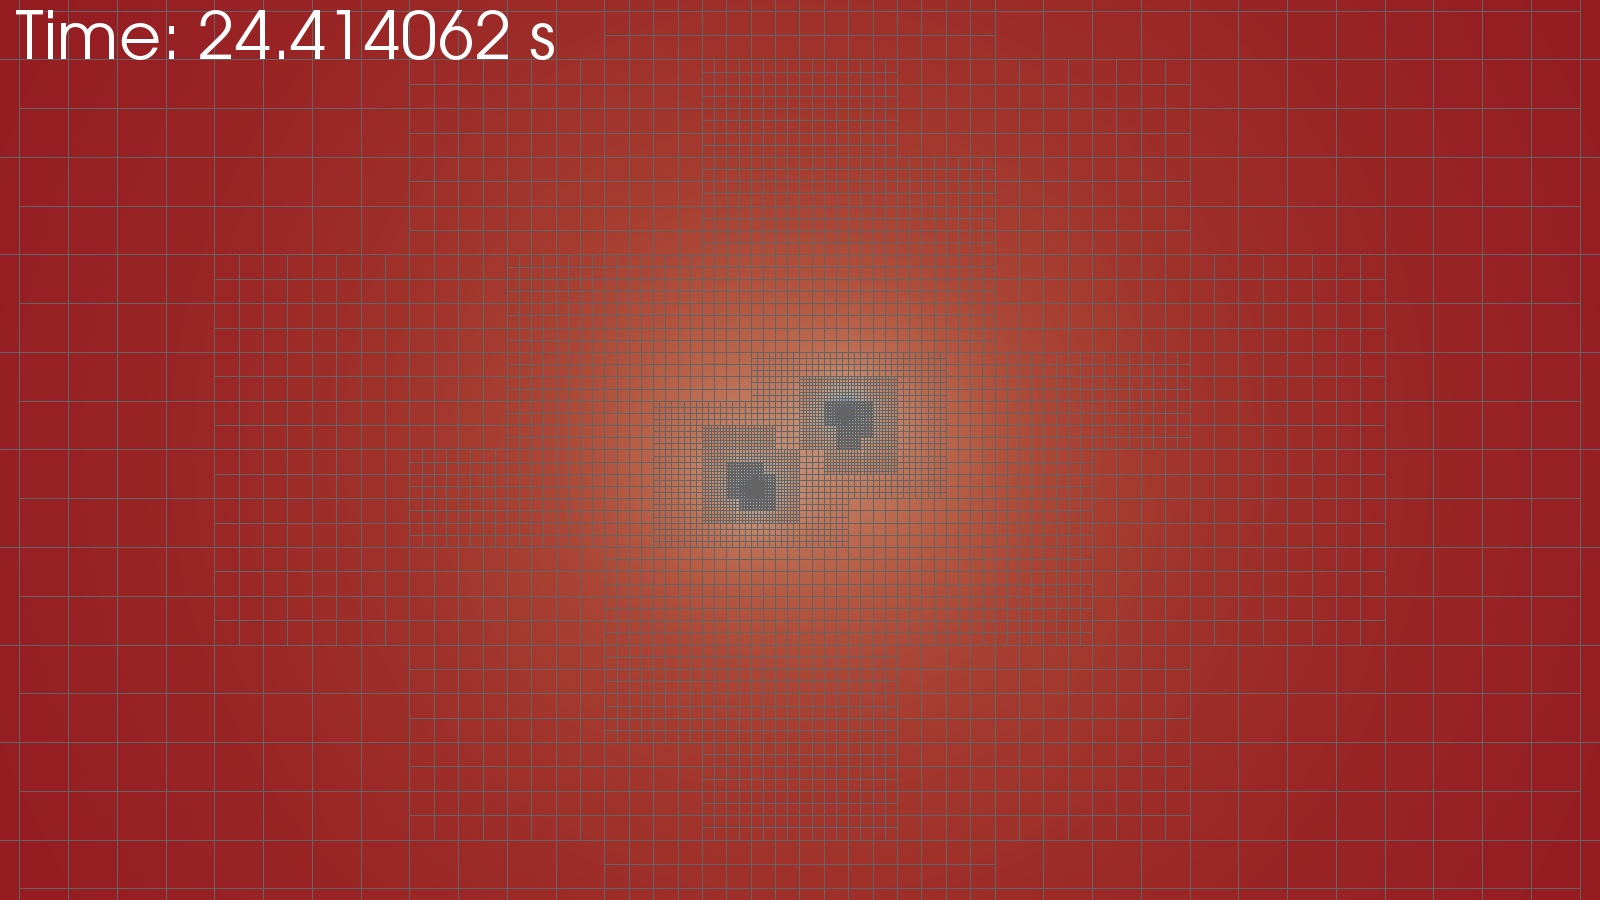
\includegraphics[width=0.22\textwidth]{figs/paraview/r1/new/img_slice_level_000200.png}
	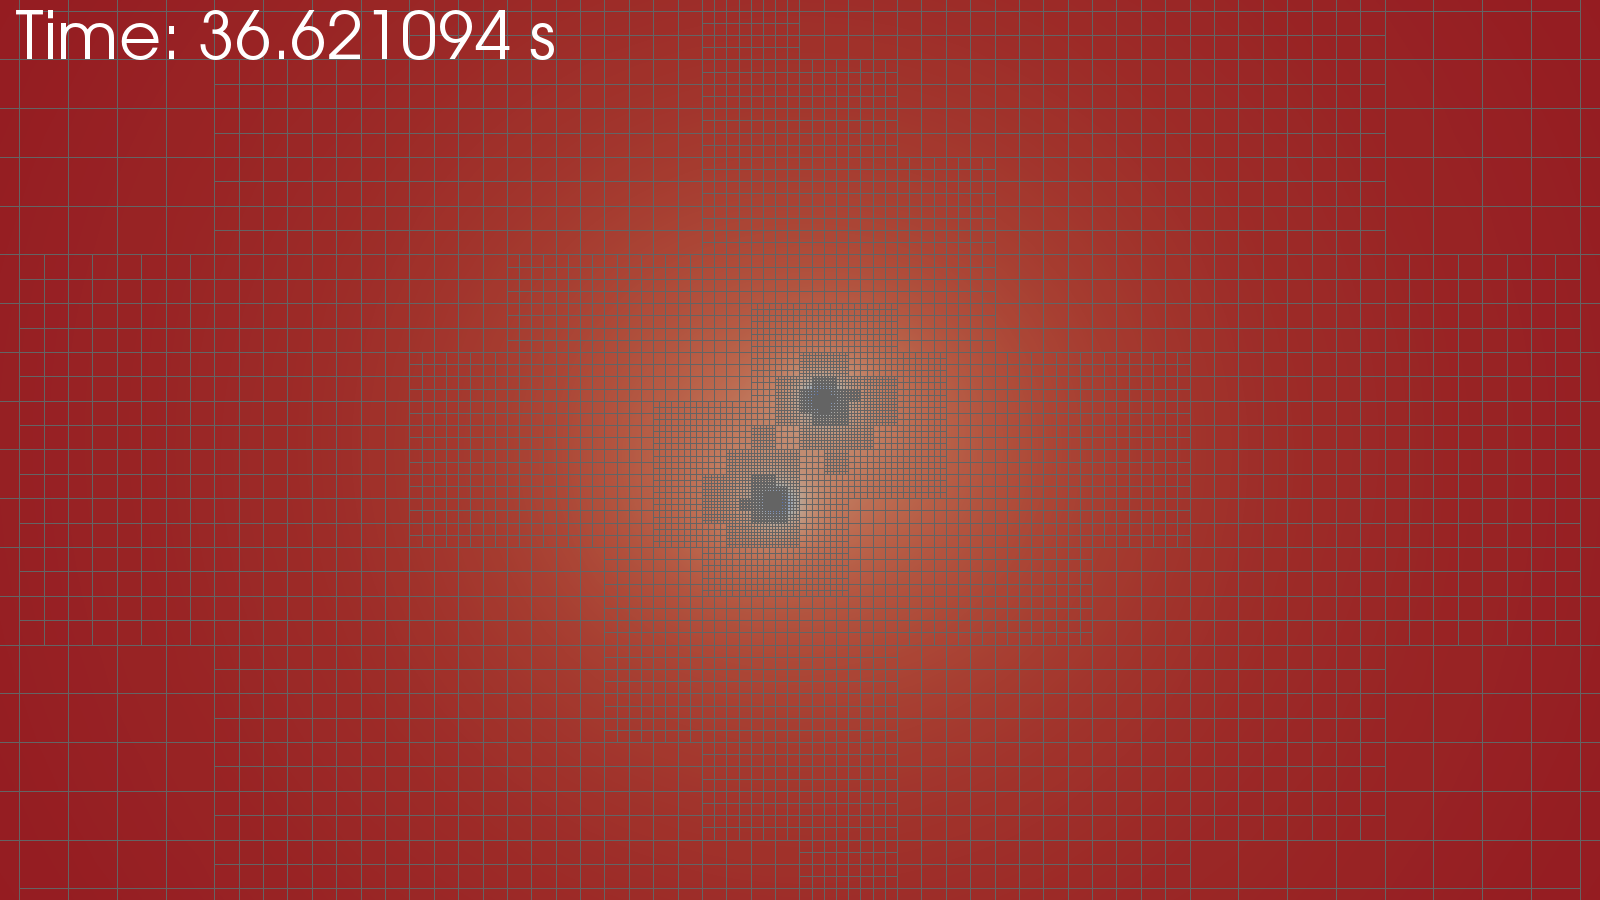
\includegraphics[width=0.22\textwidth]{figs/paraview/r1/new/img_slice_level_000300.png}
	\hfill
	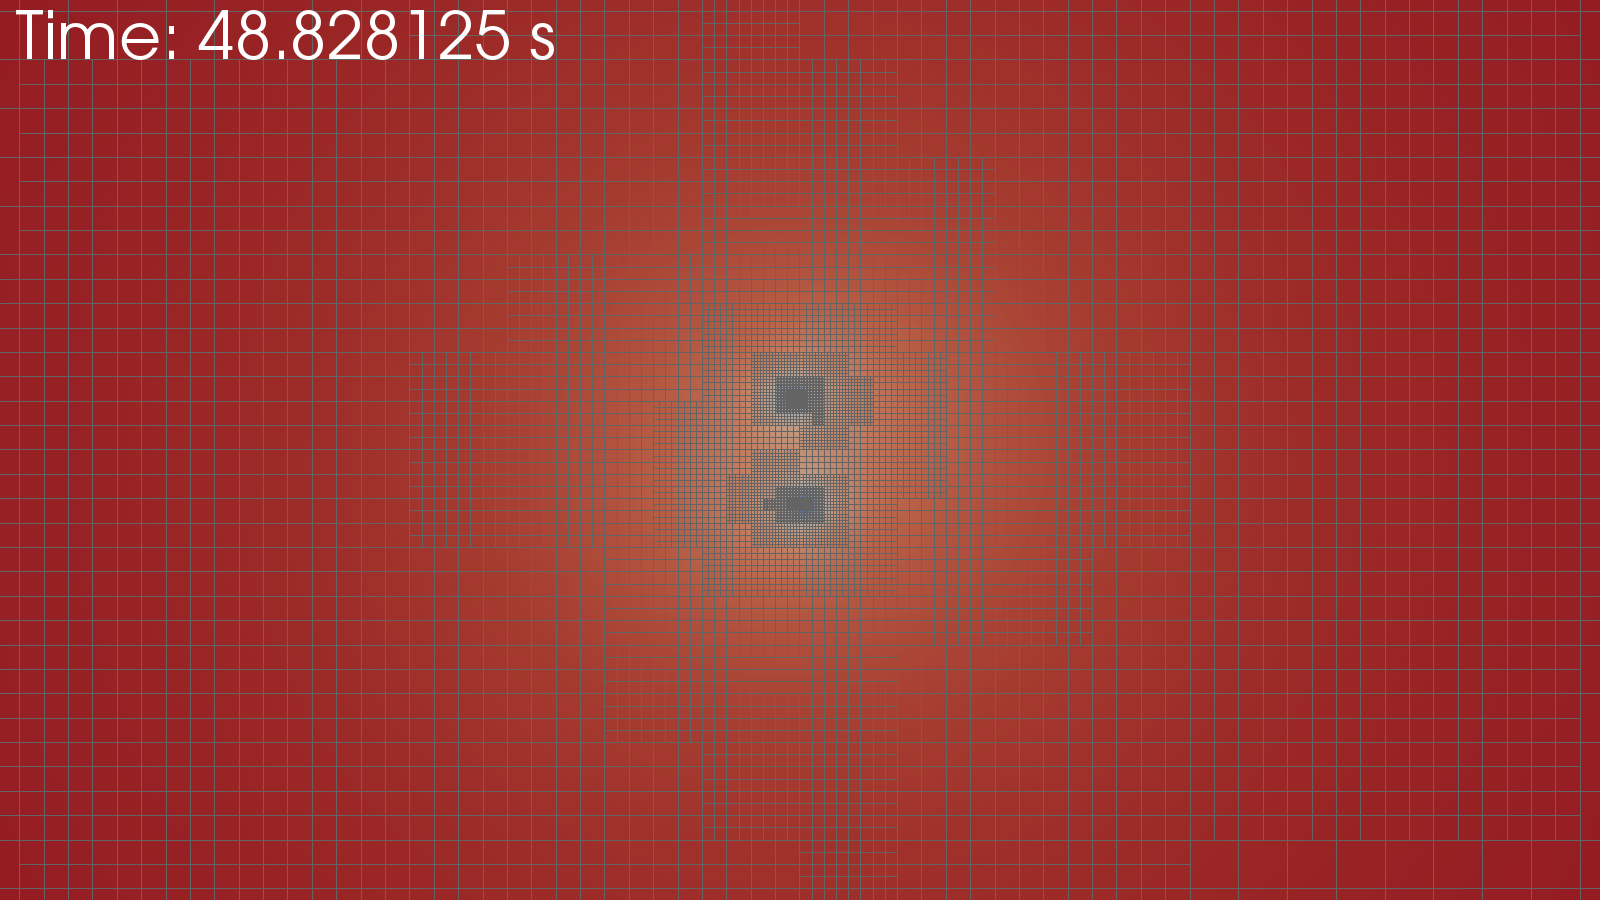
\includegraphics[width=0.22\textwidth]{figs/paraview/r1/new/img_slice_level_000400.png}	
	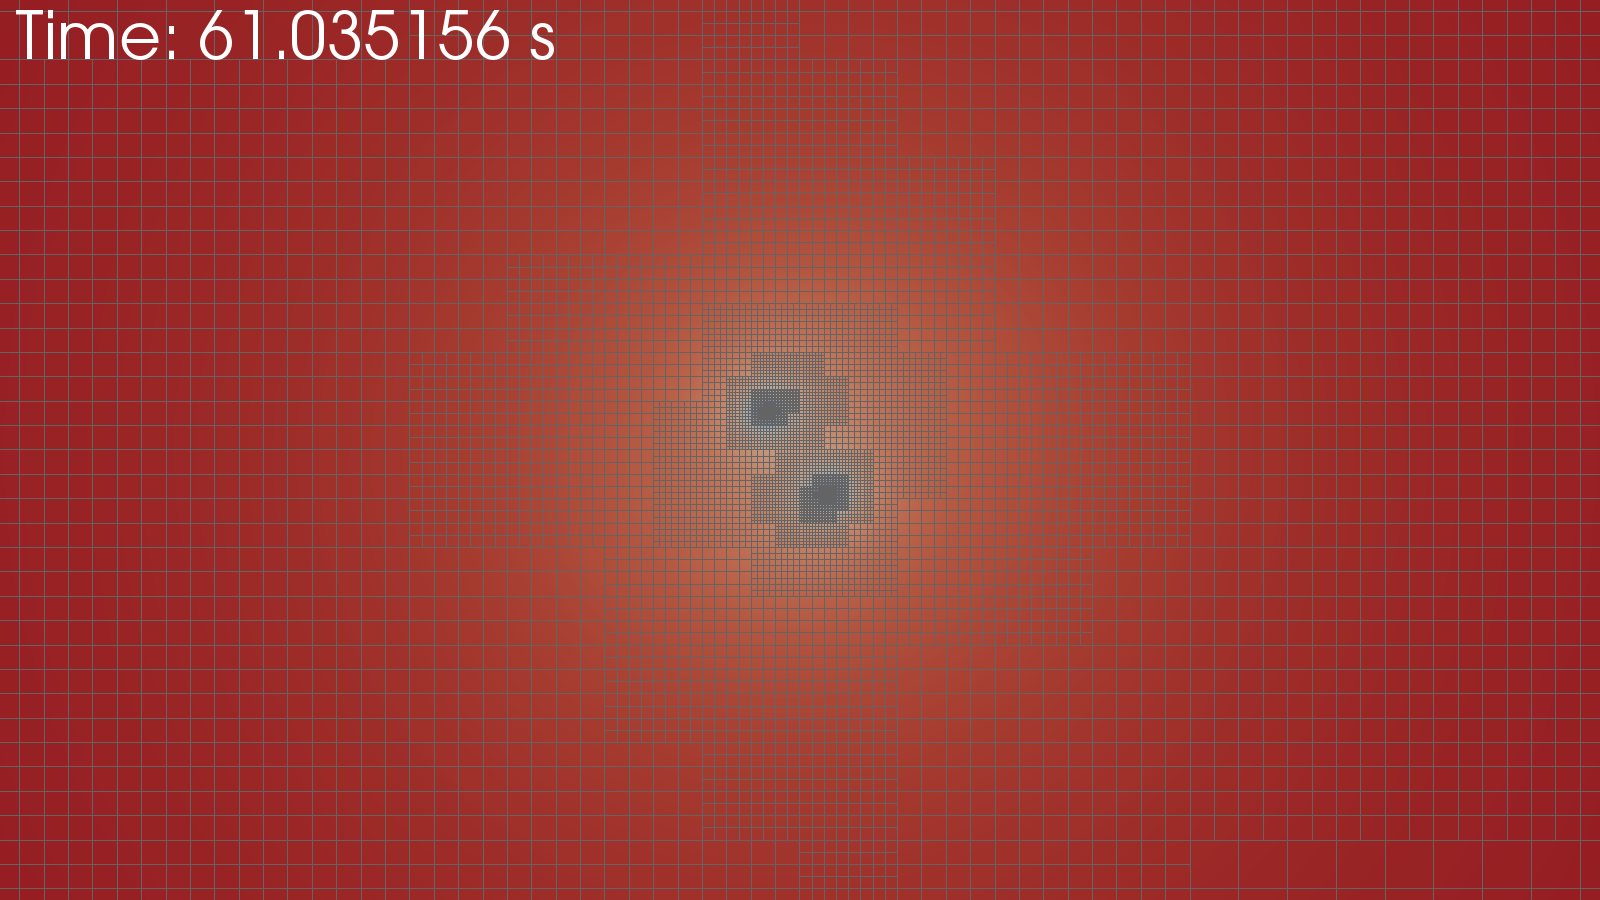
\includegraphics[width=0.22\textwidth]{figs/paraview/r1/new/img_slice_level_000500.png}	
	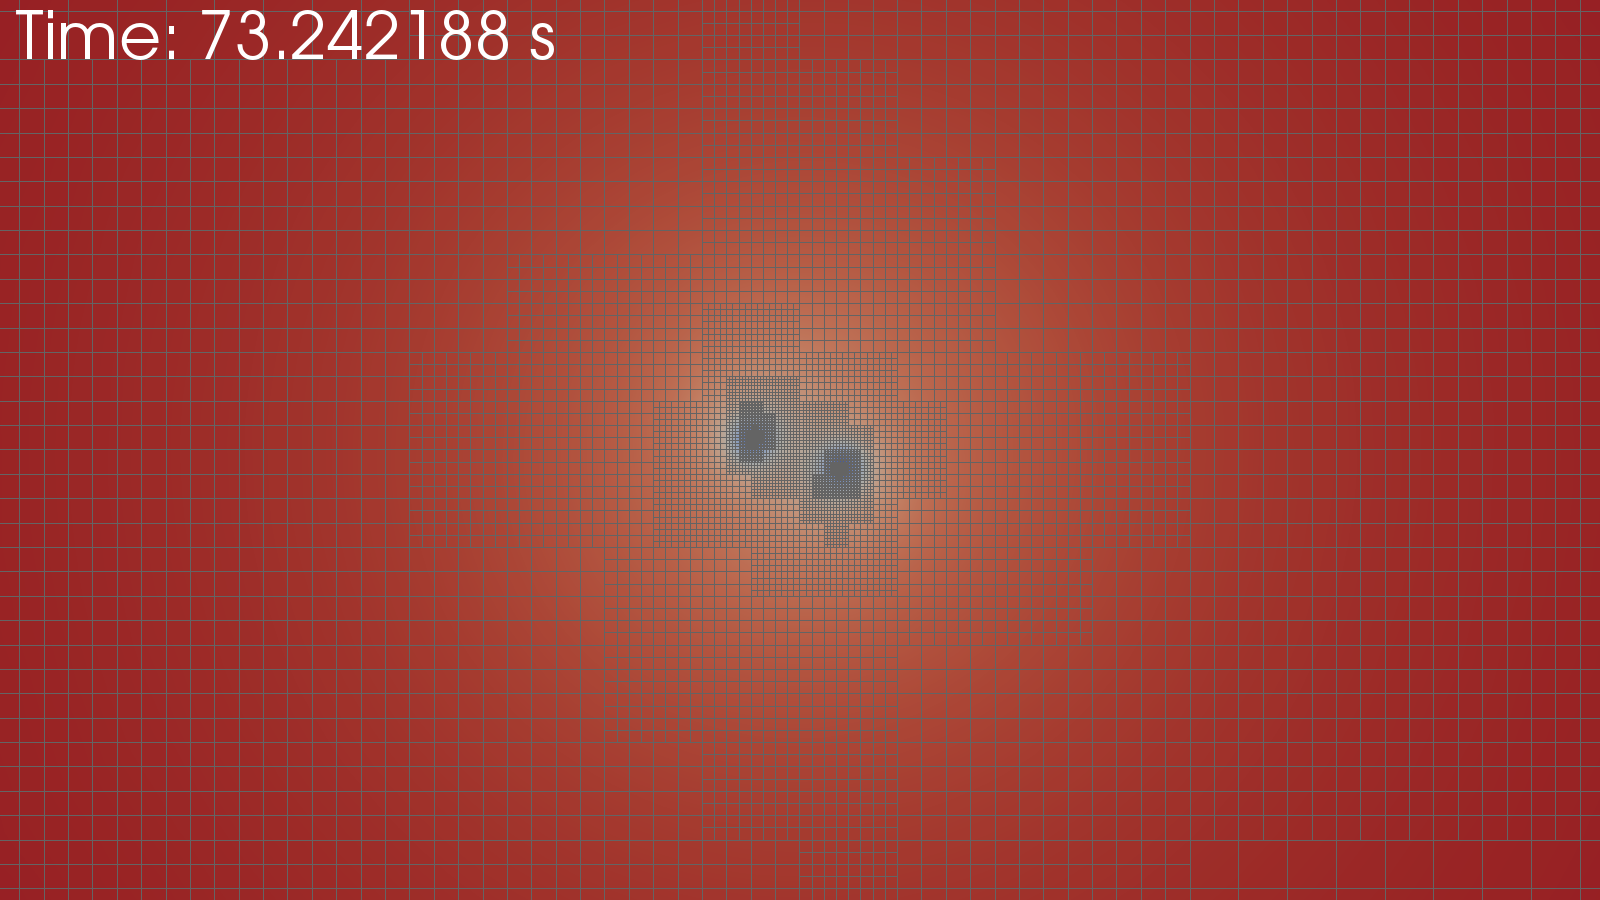
\includegraphics[width=0.22\textwidth]{figs/paraview/r1/new/img_slice_level_000600.png}	
	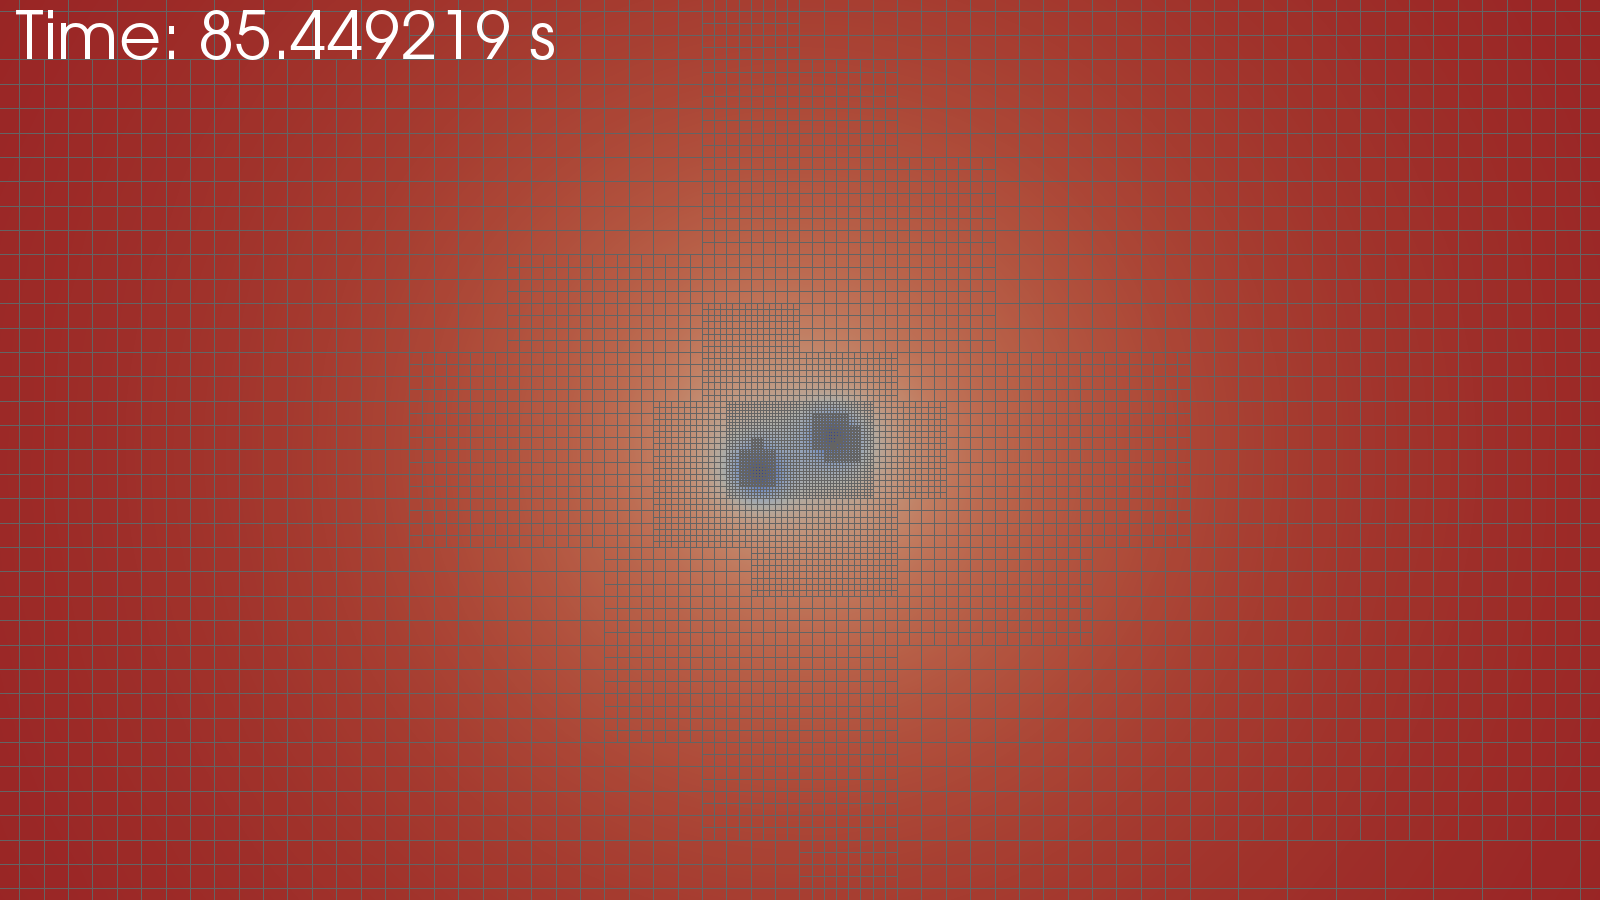
\includegraphics[width=0.22\textwidth]{figs/paraview/r1/new/img_slice_level_000700.png}	
	\hfil
	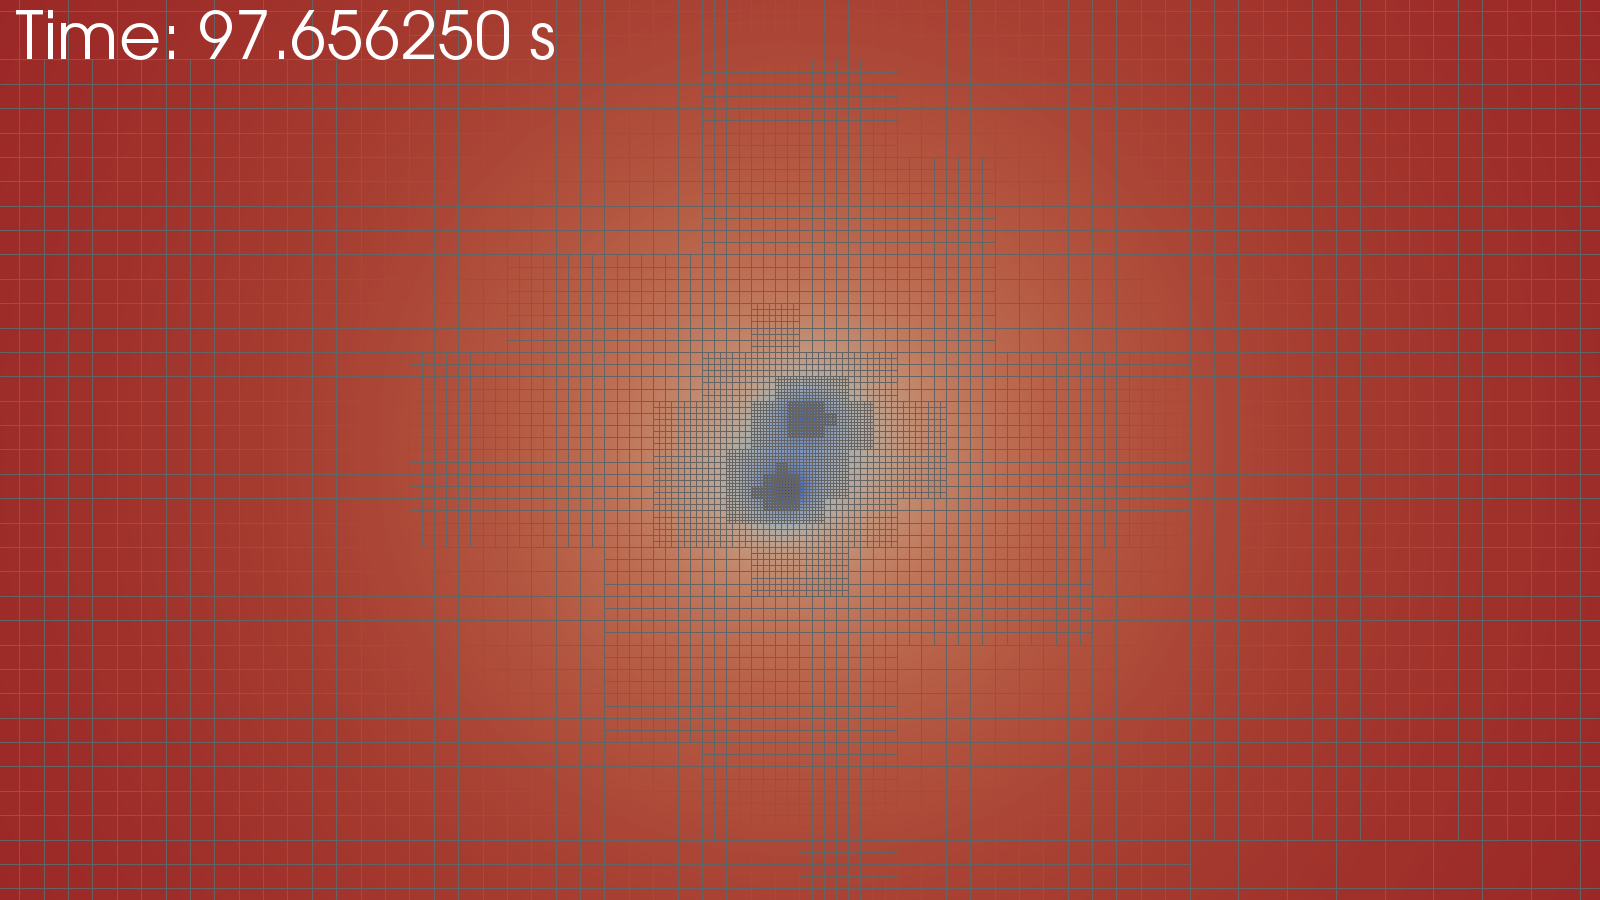
\includegraphics[width=0.22\textwidth]{figs/paraview/r1/new/img_slice_level_000800.png}	
	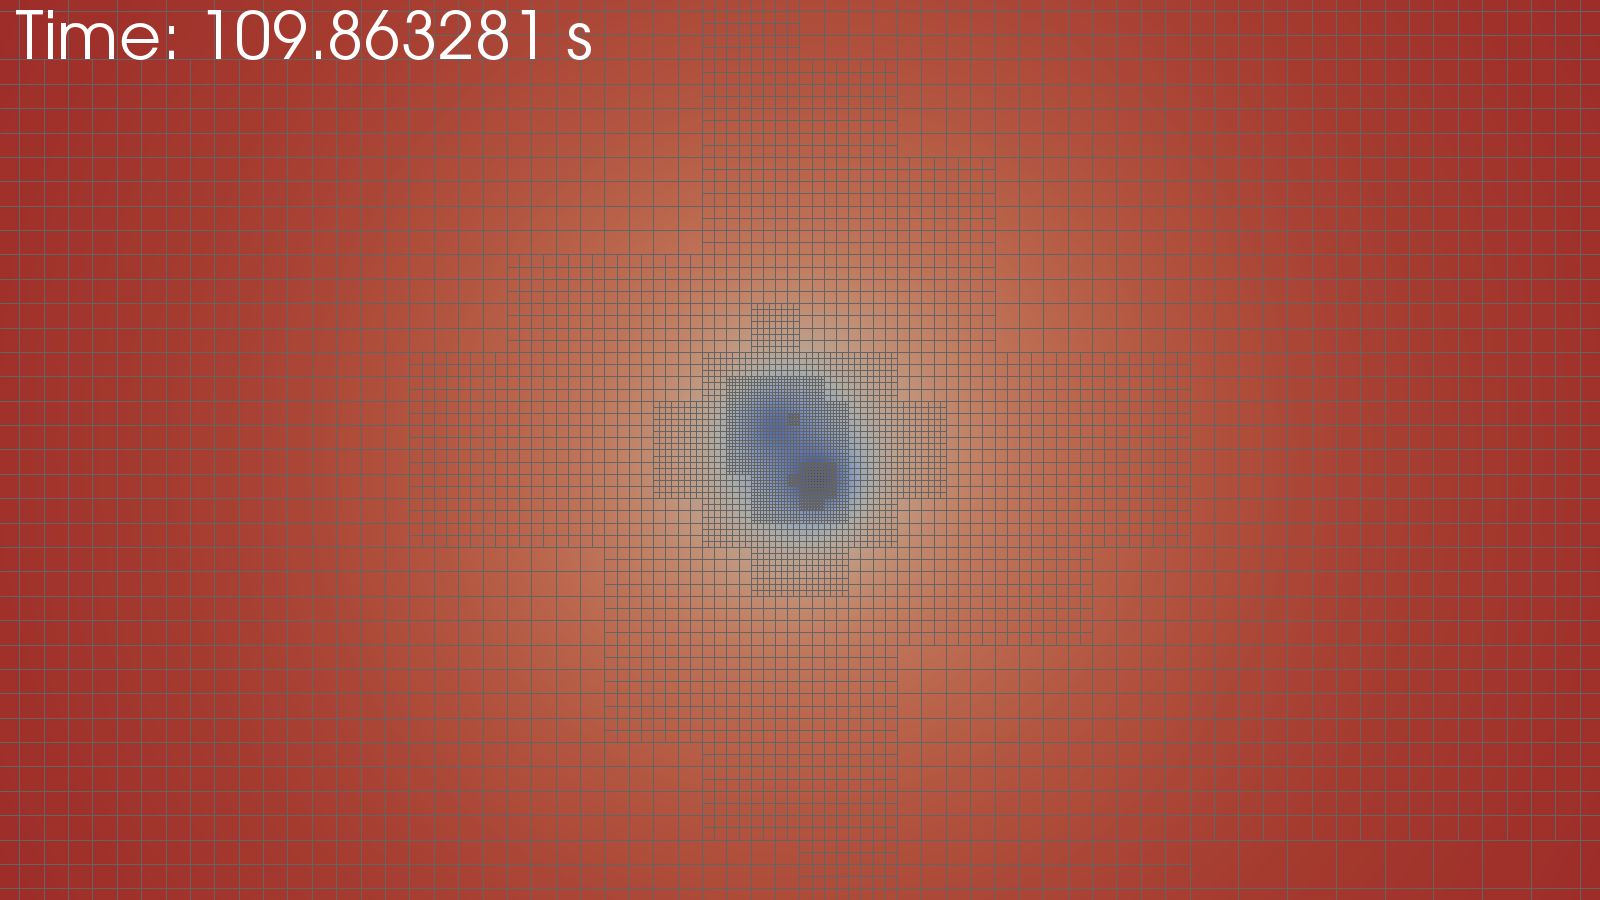
\includegraphics[width=0.22\textwidth]{figs/paraview/r1/new/img_slice_level_000900.png}	
	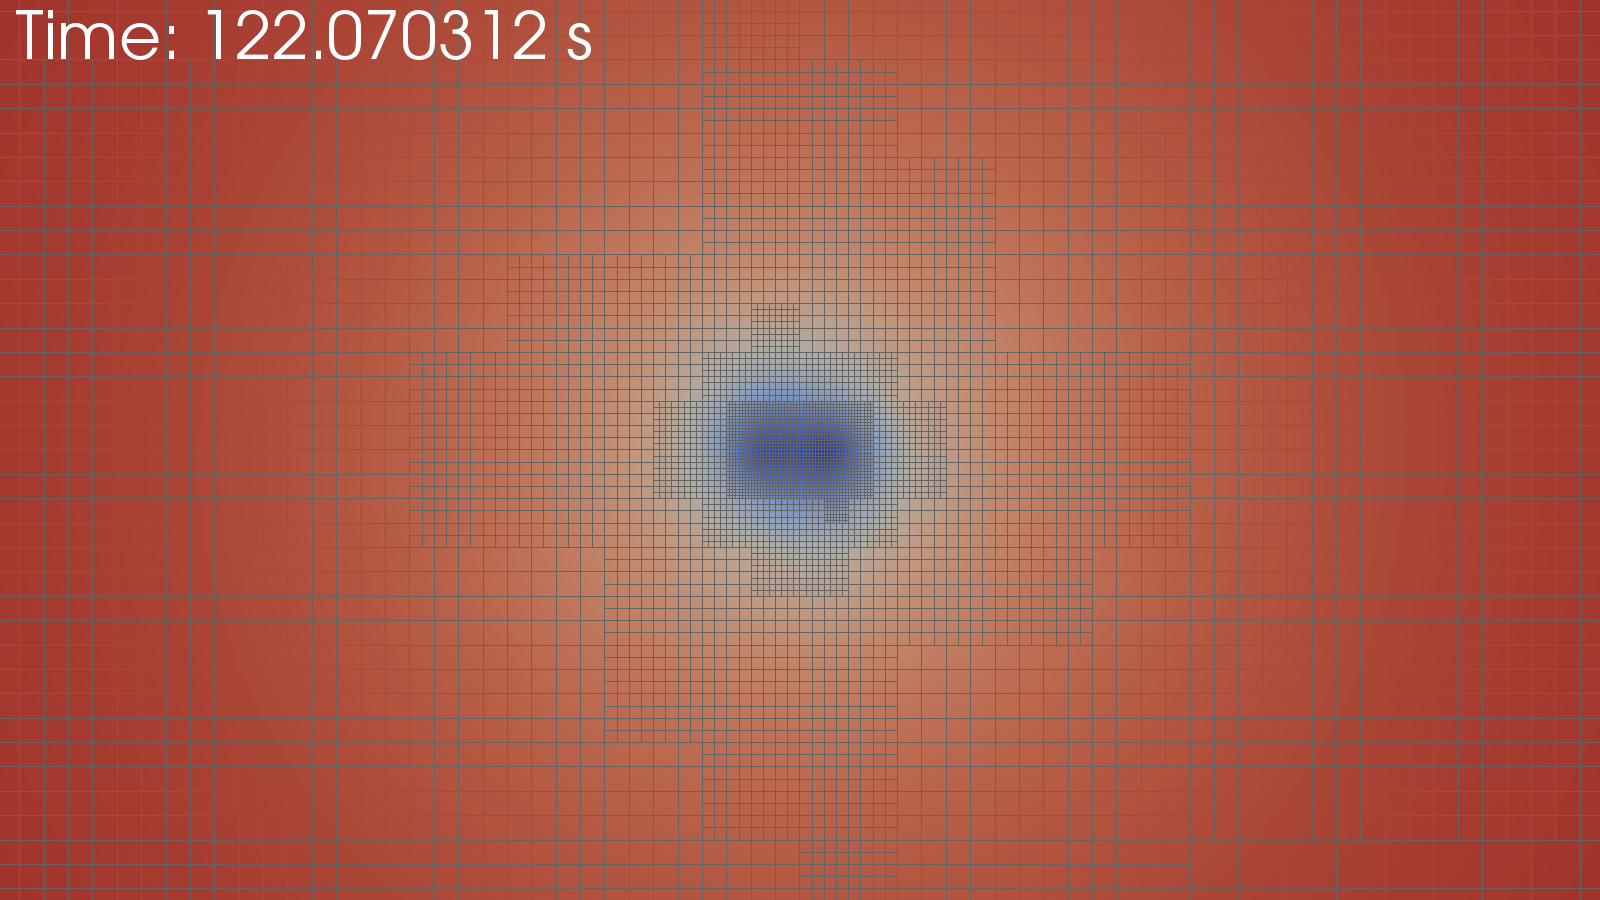
\includegraphics[width=0.22\textwidth]{figs/paraview/r1/new/img_slice_level_001000.png}	
	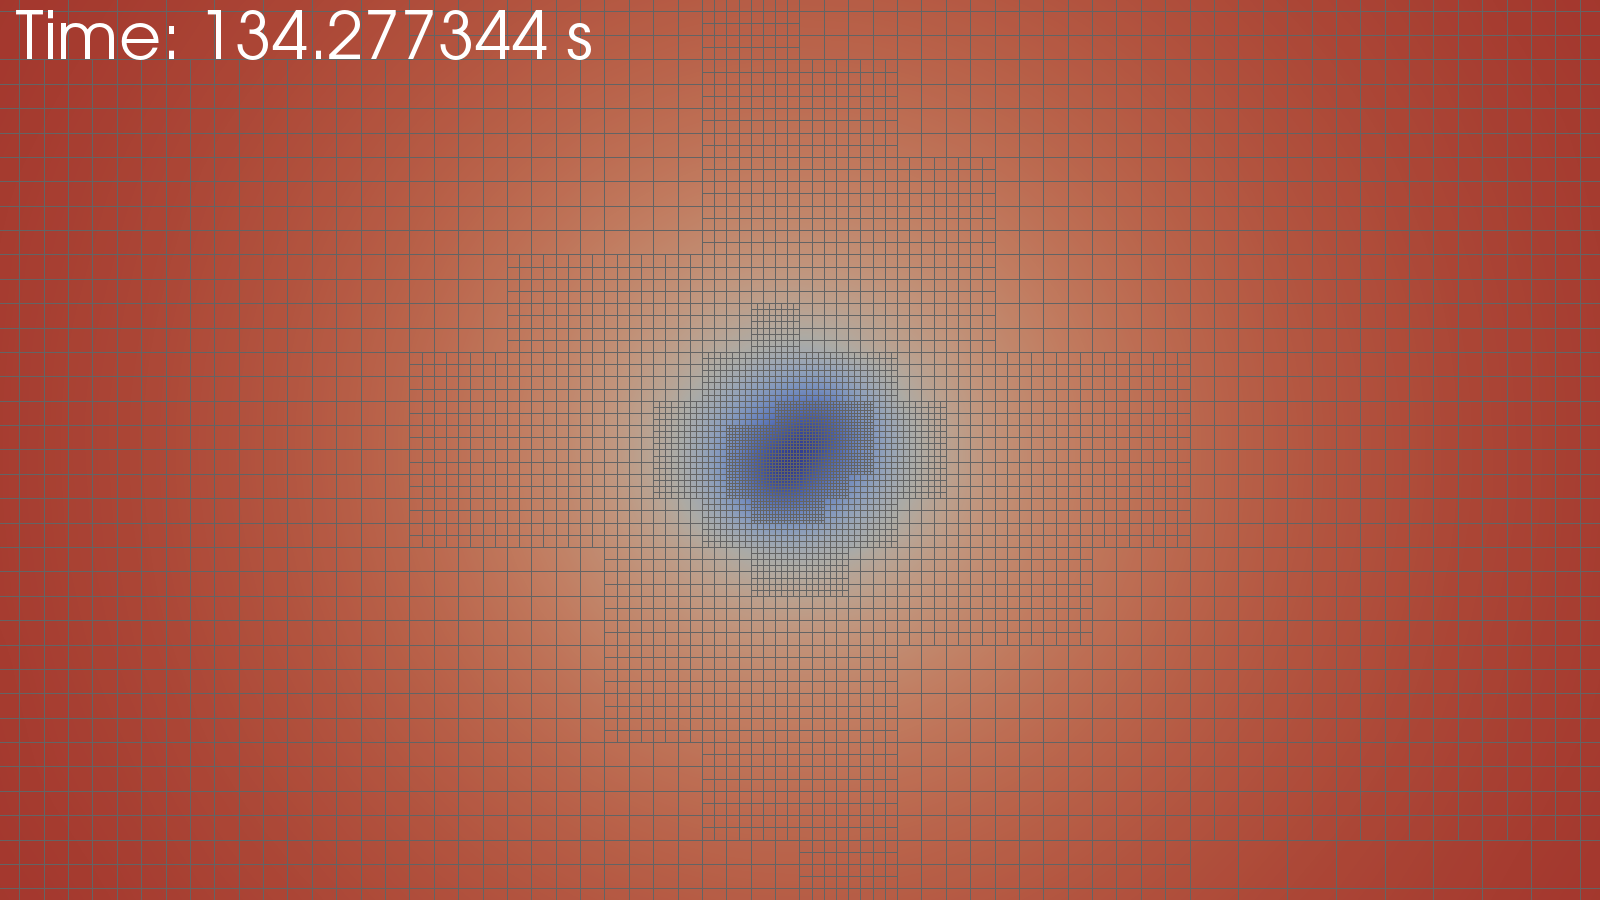
\includegraphics[width=0.22\textwidth]{figs/paraview/r1/new/img_slice_level_001100.png}	
	\caption{WAMR (cell refinement level) for equal mass ratio black hole merger simulation with maximum refinement level of $14$ with wavelet tolerance of $10^{-4}$ perfomred in CHPC \label{fig:pv:r1_level}}
\end{figure}



We will provide the final version of the ParaView python script (\texttt{bssnVis.py}) for the project evaluation. We believe that the ParaView batch mode based visualization almost finished but new filters and pipelines can be setup as needed.
Note that we can use paraview trace mode to generate the basic code structures for new filters and modify them as needed. 

\subsection{VTK based visualization }
Visualization ToolKit (VTK) is one of the most powerful, scalable visualization package that is mainly developed by KitWare and Sandia National Laboratory. ParaView is a GUI which is build upon VTK, ParaView does have almost the basic functions, 
in VTK but there are some VTK functionalities that is not present in ParaView (i.e. Gradient Opacity Transfer functions). VTK is primarily supports in C/C++ there are some wrappers for other languages such as python tcl etc. In the VTK based visualization 
we are trying to perform the same visualizations that we have done using ParaView in parallel rendering mode. We believe this is give us deeper understanding of ParaView workflow and pipeline. 

VTK based frame work contain four main scripts those are, 
\begin{itemize}
	\item \texttt{filters.py} : contains all the filters needed for visualization
	\item \texttt{vtkio.py}: contains IO utilities
	\item \texttt{render.py} : contains render utilities
	\item \texttt{GRVis.py} : main script with puts everything together. 
\end{itemize}

\subsection{Parallel processing with VTK}
VTK has different readers for each file format. Parallel processing and rendering capability will depend on the file format the data is written. All the file formats which are written in partioned data format can be processed in parallel (i.e. reading, applying filters etc. )
and can be rendered using VTK CompositeManger in parallel. 

\subsection{Sequential rendering with VTK}
Compared to paraview based scripting VTK is more primitive and has more flexibility for the programmer. Overall VTK visualization pipeline is you can read input data form VTK supported file format with the corresponding reader. Then user can program required filters which can be passed to the rendering process. Rendering in VTK slightly more complicated compared to paraview since paraview has automated this process for the user. In VTK rendering, first user need to create a \texttt{Mapper} which take some file input connection to known topology mapping to VTK (i.e. map input to polygonal data), and it is reuired that the file is written in the correct format to perform this mapping correctly. Once we have an \texttt{Mapper} we can create an \texttt{Actors} for everything needed to be rendered in the rendering window. We can add multiple actors to renderer and we can create a rendering window using the renderer. 

\subsection{Parallel rendering with VTK}
VTK supports parallel distributed memory rendering which can be essential with dealing with large data sets. In order to perform parallel rendering, we need use, \texttt{vtkCompositeRenderManager} which we can then add multiple render windows and set the primary render window to render the final image. Following is an example of using \texttt{vtkCompositeRenderManager}.

\begin{lstlisting}[language=Python]
compManager = vtk.vtkCompositeRenderManager()
if compManager.GetController():
 rank = compManager.GetController().GetLocalProcessId()
 npes = compManager.GetController().GetNumberOfProcesses()
else:
 print("Error "+str(renderGeometry.__name__)+" in VTK composite manager")        
 sys.exit()

'''
 Read file apply filters and create mappers and actors and render windows. 
'''	 
if npes > 1 and useParallelRendering:
 compManager.SetRenderWindow(renderer_window)
 compManager.InitializePieces()

if rank == 0:
 iren = vtk.vtkRenderWindowInteractor()
 iren.SetRenderWindow(renderer_window)
 iren.AddObserver("ExitEvent", ExitMaster)
 iren.Initialize()
 iren.Start()
else:
 compManager.InitializeRMIs()
 compManager.GetController().ProcessRMIs()
 compManager.GetController().Finalize()
 #print "**********************************"
 #print "Done on the slave node"
 #print "**********************************"
 sys.exit()
\end{lstlisting}


In order to read \texttt{.pvtu} files we use, \texttt{vtkXMLPUnstructuredGridReader} which performs the parallel processing internally transparent to the user. Reading the \texttt{.pvtu} file can be done as follows. 
\begin{lstlisting}[basicstyle=\small]
''
@brief Reads the XML partioned unstructed 
grid and retuns, vtkXMLPUnstructuredGridReader
'''
def ReadPVTUFile(fname):
reader=vtk.vtkXMLPUnstructuredGridReader()
reader.SetFileName(fname)
reader.Update()
#print reader.GetNumberOfPieces()
return reader
\end{lstlisting}

In order to benefit from the parallelism we need to run VTK using MPI, this can be performed using \texttt{MPI4Py} and \texttt{pvtkpython} which enables us to run the VTK in distributed mode as follows.
\begin{lstlisting}[basicstyle=\small]
mpirun -np 8 pvtkpython <VTK script>
\end{lstlisting} 

At this point we have performed slice through the data and visualize the BSSN variable $\chi$ over the slice, an generated figure is shown in Figure \ref{fig:vtk:r1}. 

\begin{figure}[H]
	\centering
	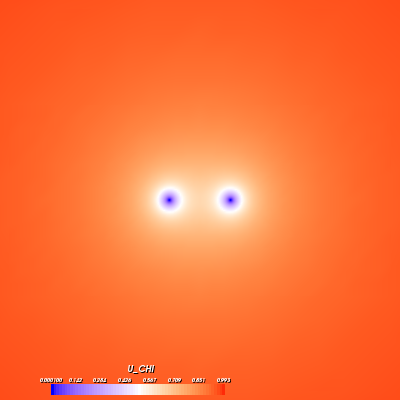
\includegraphics[width=0.18\textwidth]{figs/vtk/r1/img_slice_000000.png}
	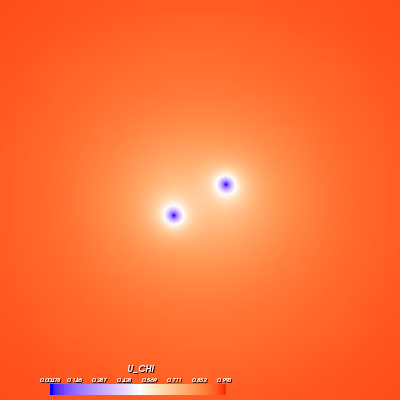
\includegraphics[width=0.18\textwidth]{figs/vtk/r1/img_slice_000020.png}
	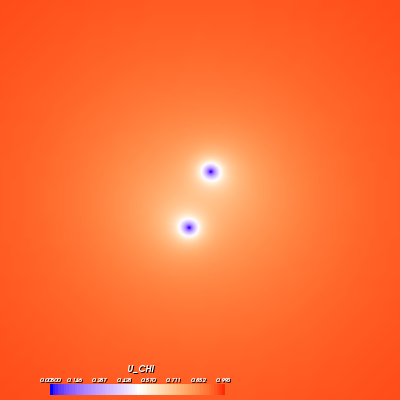
\includegraphics[width=0.18\textwidth]{figs/vtk/r1/img_slice_000040.png}
	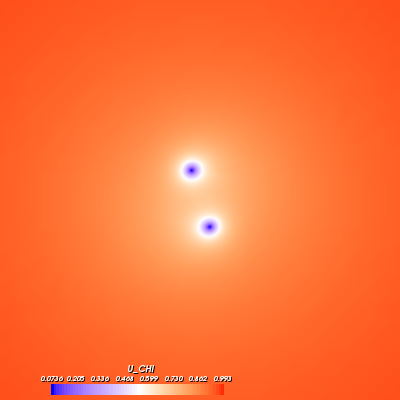
\includegraphics[width=0.18\textwidth]{figs/vtk/r1/img_slice_000060.png}
	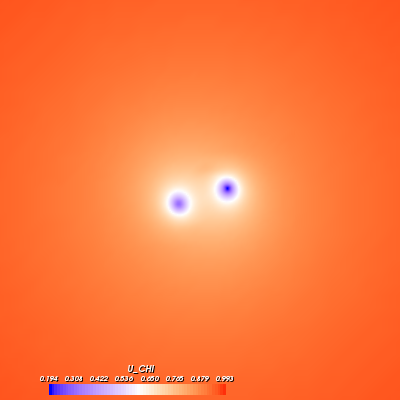
\includegraphics[width=0.18\textwidth]{figs/vtk/r1/img_slice_000100.png}
	\caption{VTK based generated time series images for bssn variable $\chi$ the equal mass ratio binary merger with maxdepth of $14$ and wavelet tolerance of $10^{-3}$ \label{fig:vtk:r1}}
\end{figure}


\begin{figure}[H]
	\centering
	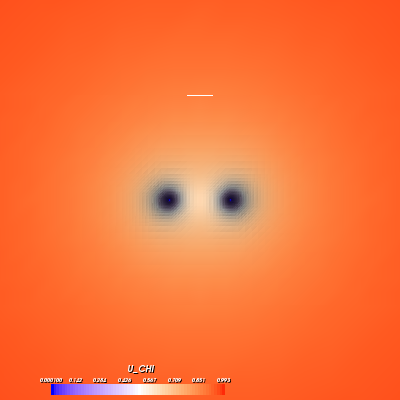
\includegraphics[width=0.18\textwidth]{figs/vtk/r1/img_slice_wbs_000000.png}
	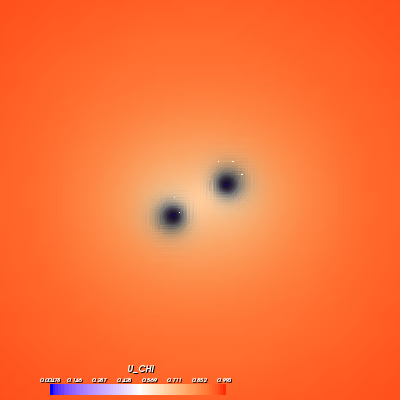
\includegraphics[width=0.18\textwidth]{figs/vtk/r1/img_slice_wbs_000020.png}
	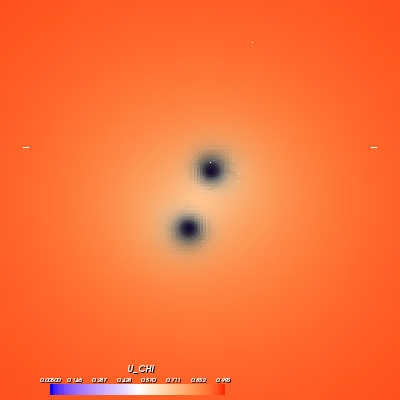
\includegraphics[width=0.18\textwidth]{figs/vtk/r1/img_slice_wbs_000040.png}
	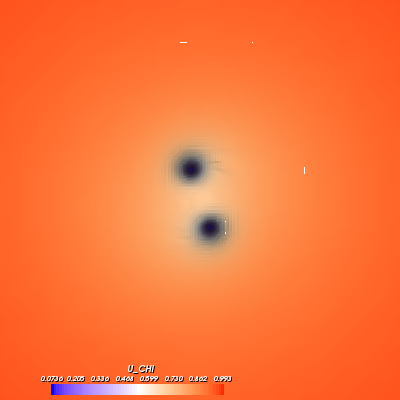
\includegraphics[width=0.18\textwidth]{figs/vtk/r1/img_slice_wbs_000060.png}
	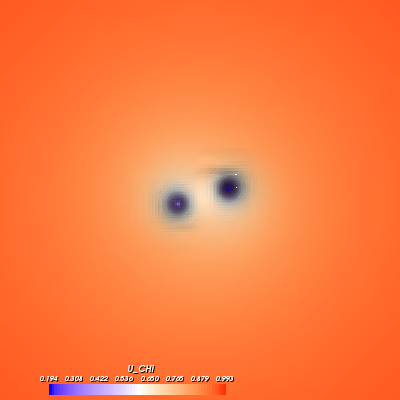
\includegraphics[width=0.18\textwidth]{figs/vtk/r1/img_slice_wbs_000100.png}
	\caption{VTK based generated time series images for bssn variable $\chi$ with warp by scalar for the equal mass ratio binary merger with maxdepth of $14$ and wavelet tolerance of $10^{-3}$ \label{fig:vtk:r1}}
\end{figure}
